\documentclass[pdflatex,sn-basic]{sn-jnl}
\usepackage{graphicx}
\usepackage{amsmath,amssymb,amsfonts}
\usepackage{booktabs}
\usepackage{longtable}
\usepackage{xcolor}
\newcommand{\fn}[1]{\texttt{\detokenize{#1}}}


\raggedbottom

\begin{document}

\title[Trustworthy AI for Low-Carbon Geopolymers]{From Property Prediction to Clean-Technology Deployment: A Systematic Review and Roadmap for Trustworthy AI in Low-Carbon Geopolymer Development}

\author*[1]{\fnm{Vinoth} \sur{Nageshwaran}}\email{vnageshwaran41452@ucumberlands.edu}
\author[2]{\fnm{Pooja Kaur} \sur{Chaggar}}
\author[3]{\fnm{Sudhir S.} \sur{Amritphale}}
\author*[2]{\fnm{Mariam} \sur{Darestani}}\email{m.darestani@westernsydney.edu.au}

\affil*[1]{\orgname{University of the Cumberlands}, \orgaddress{\city{Williamsburg}, \state{KY}, \country{USA}}}
\affil[2]{\orgname{Western Sydney University}, \orgaddress{\city{Kingswood}, \state{NSW}, \country{Australia}}}
\affil[3]{\orgname{Science Investments LLC (formerly Louisiana Tech University)}, \orgaddress{\city{Ruston}, \state{LA}, \country{USA}}}

\abstract{Geopolymers made from industrial residues are a credible low-carbon alternative to Portland cement, and artificial intelligence (AI) is widely expected to speed their development. This systematic review asks how far published AI-enabled geopolymer research has moved from predicting single properties toward models that are trustworthy, physically grounded, environmentally quantified and usable in practice. Following PRISMA 2020, 894 unique records were screened and 728 included, representing 669 unique primary journal studies (2013--2026); 71\% were published after the closest prior review. Each study was coded on a six-axis framework by a deterministic keyword classifier applied to its title, abstract and keywords, and three subsets were audited in more detail. Because keyword coding of abstracts under-detects practices reported only in full text, corpus-wide shares are provisional and trust-practice shares are lower bounds. Prediction and optimization make up 94.5\% of the corpus. Explainability is signalled in 39.3\% of studies, whereas external validation (4.6\%), uncertainty quantification (1.8\%) and calibration (0.6\%) are rarely signalled and no abstract names a code repository. Of 32 studies audited for claimed or implied physics- or chemistry-informed learning, 11 were verified (nine at mix level, two atomistic) and 18 were downgraded. At least 41\% of studies mention no environmental variable, and two studies report a boundary-explicit life-cycle assessment. No physical closed-loop experiment, digital twin or certification pathway was detected. Nine research gaps with acceptance criteria and a staged roadmap follow, with implications for journals, standards bodies and environmental policy. The coded corpus is openly archived.}

\keywords{geopolymer, alkali-activated materials, machine learning, trustworthy AI, life-cycle assessment, low-carbon construction}

\maketitle

\section{Introduction}\label{sec:intro}

\subsection{The problem}

Cement production accounts for roughly seven to eight percent of anthropogenic CO$_2$ emissions. Geopolymers and the wider family of alkali-activated materials (AAMs) are among the most studied substitutes: they can lower embodied carbon relative to Portland cement and they consume industrial residues such as fly ash, slag, red mud and mine tailings. Their difficulty is variety. AAMs are a large family of materials made from feedstocks that differ between regions, plants and batches, under many activation and curing conditions. Trial-and-error mix development, which was adequate for a standardized product like Portland cement, is slow for such a family.

Artificial intelligence (AI), and machine learning (ML) in particular, is the tool most often proposed to remove this bottleneck. Over the past decade a large literature has applied ML to predict geopolymer properties, to explain the predictions, to optimize mixes and, in prospect, to plan experiments automatically. Whether ML can fit geopolymer data is no longer in doubt. The open question for clean technology is different: can these models be relied on, outside the data they were trained on, to design low-carbon materials that reach construction practice?

\subsection{The gap in existing reviews}

Earlier reviews of AI in geopolymer research are useful catalogues. They organize the literature by algorithm or by predicted property, and the most systematic of them covers 184 studies published up to December 2023 \citep{nguyen2025}. A further systematic review surveys the algorithms and statistical models used for geopolymer strength prediction \citep{matsimbe2024}. Three things are missing. First, most of the literature is newer than these reviews: 71\% of the studies analyzed here appeared from January 2024 onward. Second, the earlier reviews report what studies say they do; none checks those statements against stated criteria. Third, beyond summaries of data quality and of post-hoc interpretability, none systematically assesses the properties that decide whether a model can support an engineering or policy decision, namely reliability of predictions, quality of environmental quantification and readiness for deployment (Table~\ref{tab:prior}).

\subsection{Objective, scope and contributions}

This review addresses one question: to what extent has published AI-enabled geopolymer research progressed from isolated property prediction toward trustworthy, physics- and chemistry-aware, environmentally quantified, adaptive and deployable material design? The scope is peer-reviewed, English-language journal studies that apply ML to geopolymers or AAMs for construction-relevant purposes. With 669 studies in fourteen years, of which most are recent, the field is large enough to be assessed as a whole and young enough for its conventions to be changed; the length of this review is fitted to that task, and per-study tables are placed in the Supplementary Materials.

The review is written to the expectations for review articles set out by this journal \citep{araujo2025}: a replicable selection process, a framework that goes beyond narrative or bibliometric description, and an account readable by newcomers that still offers something new to specialists. It makes four contributions. (1) A systematically selected, openly released corpus of 669 studies with a documented screening record. (2) A six-axis framework that codes each study by material, AI task, trust practices, physics integration, environmental function and deployment maturity. (3) Three focused audits, of trust practices, of physics-integration claims and of environmental claims, which separate what is stated from what is demonstrated. (4) Nine research gaps with acceptance criteria and a staged roadmap, with recommendations for journals, standards bodies and policy makers. The trust dimensions used here overlap with existing reporting guidance for ML in concrete science \citep{li2022} and for ML-based science in general \citep{kapoor2024}; this review applies them as an audit of a published literature and not as a checklist for authors.

Section~\ref{sec:methods} describes the review methodology, including the research questions, the search, the eligibility criteria and who and what performed the screening and coding. Section~\ref{sec:background} gives background for readers new to either geopolymers or ML. Section~\ref{sec:framework} presents the framework, Section~\ref{sec:findings} the findings, Section~\ref{sec:gaps} the gaps and roadmap, Section~\ref{sec:policy} the policy implications and Section~\ref{sec:limits} the limitations.

\begin{table}[htbp]
\caption{Prior reviews at the AI $\times$ geopolymer intersection compared with this review}\label{tab:prior}
\centering
{\footnotesize
\begin{tabular}{p{0.13\textwidth}p{0.18\textwidth}p{0.12\textwidth}p{0.12\textwidth}p{0.13\textwidth}p{0.11\textwidth}}
\toprule
Review & Corpus and window & Trust assessed & Physics claims assessed & Environmental claims assessed & Systematic selection \\
\midrule
\citet{nguyen2025} & 184 studies, to Dec 2023 & partly (data quality) & no & no & yes \\
\citet{zheng2025} & narrative & interpretability only & conceptual framing & no & no \\
\citet{rathnayaka2024} & fly-ash geopolymer strength only & no & no & no & partly \\
\citet{ali2024} & several eco-concretes & no & no & no & yes \\
\citet{alaneme2023} & geopolymer concrete production & no & no & no & no \\
This review & 669 unique studies, to Aug 2026 & eight-dimension scorecard & five-level audit of 32 flagged studies & evidence ladder for 77 studies & yes, with independent verification \\
\bottomrule
\end{tabular}}
\end{table}

\section{Systematic review methodology}\label{sec:methods}

\subsection{Protocol and reporting standard}\label{sec:protocol}\label{sec:dup}

Four corpus labels are used consistently throughout this paper, and we fix them first. The \emph{screening pool} is the 894 unique records identified and screened. The \emph{Core Corpus} is the 728 included records, which represent \emph{669 unique primary studies}; unless otherwise stated, every proportion in this paper is computed on $n = 669$. The \emph{Context Corpus} is the 59 reviews and adjacent-field items (58 routed at screening and one review moved after the freeze) that inform interpretation and are never counted in the totals. The \emph{audited subsets} are the three groups examined study by study: 32 studies flagged for physics or chemistry integration, 77 studies engaging with carbon or life-cycle assessment, and 16 studies extracted from full text. Specific claims about individual studies rest on the audited subsets; the corpus-wide map supplies aggregate trends.

Two boundary conditions of the evidence base are stated here, up front, because they govern how every downstream count should be read. First, \emph{assurance differs by step}. Every one of the 894 records was screened twice, by the first author and independently by a co-author (Cohen's $\kappa = 0.83$ and 0.69; Section~\ref{sec:reliability}). The coding of the included studies, by contrast, was not done by hand: it is the output of a deterministic keyword-heuristic classifier applied to titles, abstracts and keywords, checked against a blind human recode of a 70-study sample. A practice that a study performs but does not name in its abstract, or names in words outside the lexicon, is therefore not counted: corpus-wide shares are provisional, shares for trust practices are lower bounds, and ``not detected'' means not detected at this depth unless stated otherwise. Second, \emph{the corpus is a reproducible sample, not a census}. It is drawn from Scopus and three supplementary sources, is limited to English-language journal articles, and excludes conference papers and preprints. All conclusions are framed as findings from this corpus and not as exhaustive measurements of the field.

The review is reported in accordance with the PRISMA 2020 statement \citep{page2021}. PROSPERO does not register materials-science reviews, so the protocol (research questions, sources, queries, eligibility criteria, screening design and coding schemes) was written and frozen before the search; it is released with the research artifact, and later deviations are disclosed below as dated amendments. Synthesis is structured and descriptive, not meta-analytic.

The protocol comprises four stages: (i) \emph{identification}, the execution of structured queries and the deduplication of the merged result set; (ii) \emph{screening}, the title-and-abstract assessment of deduplicated records against the criteria of Section~\ref{sec:criteria}; (iii) \emph{eligibility}, the full-text or full-abstract assessment of records that could not be resolved at screening; and (iv) \emph{inclusion}, the coding of eligible records under the framework of Section~\ref{sec:framework}. The corresponding flow is reported in Fig.~\ref{fig1}: 1,214 records identified, 320 duplicates removed and 894 screened, of which 70 were removed at title--abstract stage and 58 were routed to the Context Corpus; 37 were excluded at the eligibility stage, leaving 729 included records, frozen on 21 August 2026. One of these was removed afterwards as a dated amendment (12 November 2026): when its abstract was retrieved for coding it proved to be a bibliometric review, and it was moved to the Context Corpus, leaving 728 included records. A duplicate audit run after the freeze (DOI matching and title-similarity matching confirmed against year and venue) found 52 pairs in which a supplementary-source record with an abbreviated title duplicated a Scopus record. A further check on 12 November 2026, in which DOIs were resolved for the supplementary-source records that lacked one, found seven more such pairs (including three that the earlier audit had judged distinct), bringing the total to 59. These are flagged, not deleted, in the released file, giving 669 unique primary studies (arithmetic reconciliation in Supplementary Table S1). All searches were executed on 10 August 2026.

Reproducibility is operationalized as a re-executable workflow wherever possible. The merge, coding and scoring steps are scripted: re-running the released keyword classifier on the Scopus export and the retrieved supplementary abstracts reproduces every corpus-wide share in this paper exactly. The search log, the screening ledger with a reason code for each record, the adjudication record, the coded corpus, the audit tables and the recode worksheets are released (Data availability).

\begin{figure}[htbp]
\centering
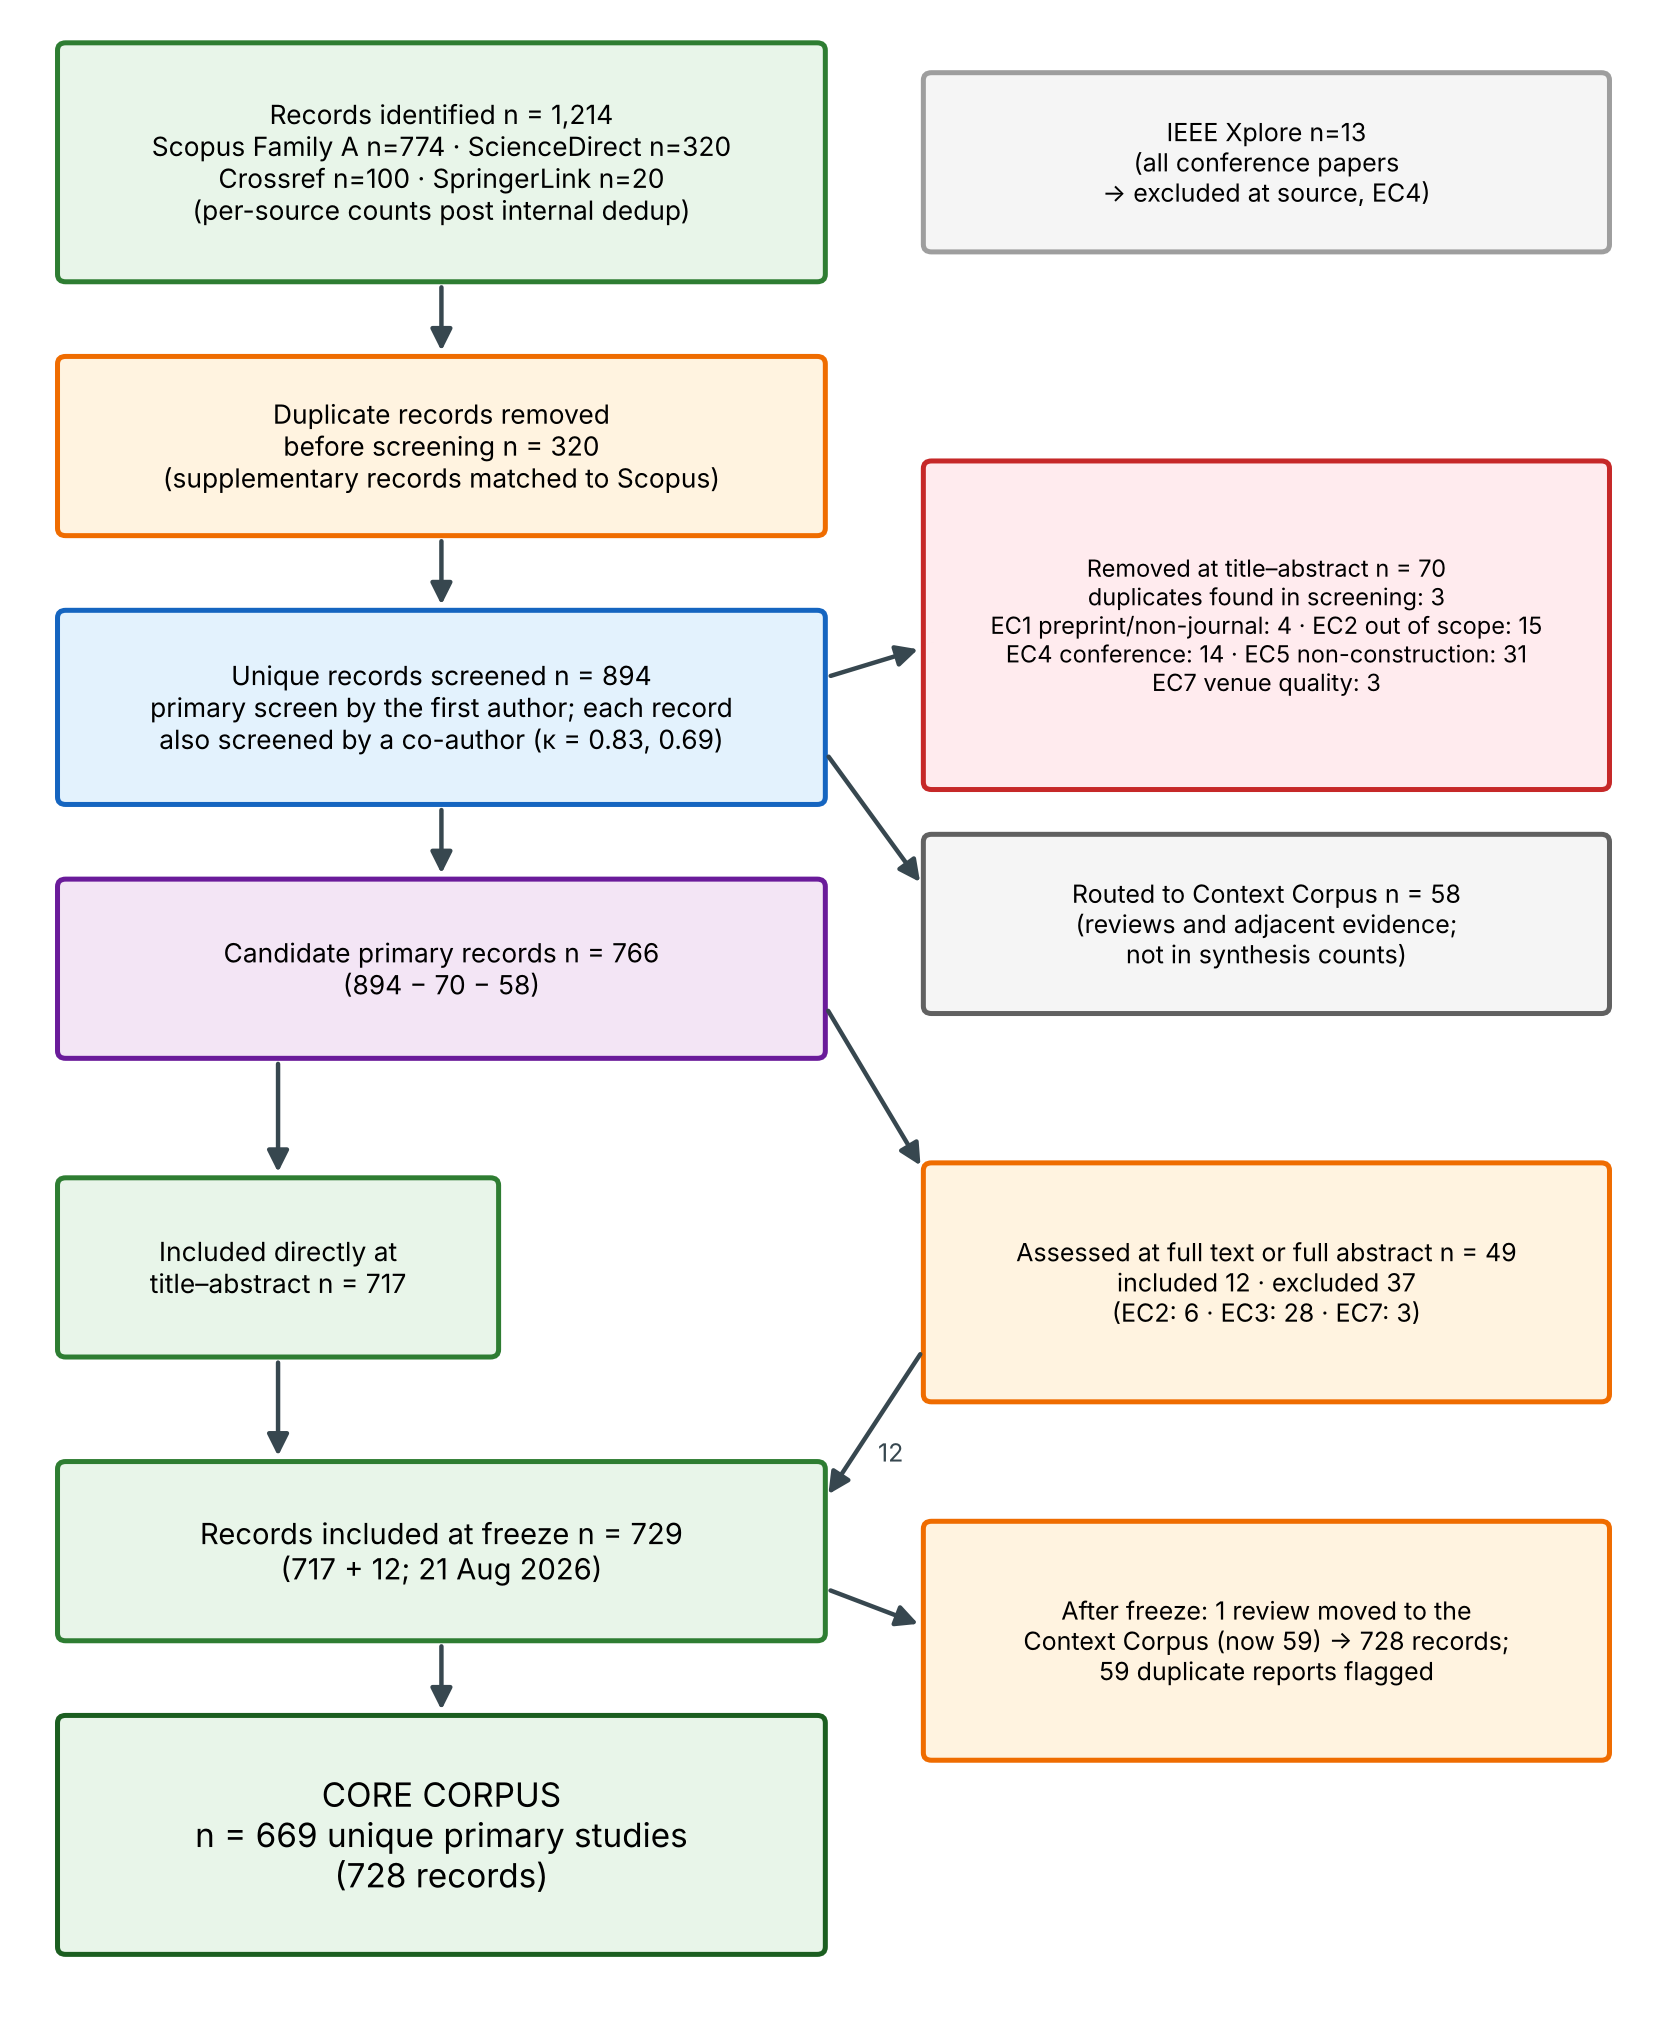
\includegraphics[width=0.85\textwidth]{Fig1.png}
\caption{PRISMA 2020 flow of study identification and selection. Each record was screened by the first author and, independently, by one of two co-authors (Section~\ref{sec:reliability}). Of the 766 candidate primary records, 717 were included directly and 49 were assessed at full text or full abstract. Stage definitions in Section~\ref{sec:protocol}; full reconciliation of counts in Supplementary Table S1}\label{fig1}
\end{figure}

\subsection{Research questions}

The protocol is organized around eight research questions that the synthesis is designed to answer (RQ1 overarching; RQ2--RQ8 thematic):

\begin{itemize}
\renewcommand\labelitemi{$\bullet$}
\item \textbf{RQ1 (Trajectory).} To what extent has published AI-enabled geopolymer research progressed from property prediction toward trustworthy, physics-aware, environmentally quantified, adaptive and autonomous design, and where does the published evidence stop?
\item \textbf{RQ2 (Materials and data).} Which precursor systems, waste streams, descriptors and datasets underpin this research, and how do dataset scale, provenance and openness limit what can be claimed?
\item \textbf{RQ3 (Environmental performance).} What share of studies quantify or optimize embodied carbon, energy, waste use, CO$_2$ uptake or life-cycle impacts, and how sound are the boundaries, data and uncertainty treatment?
\item \textbf{RQ4 (Trustworthiness).} How interpretable, uncertainty-aware, calibrated, externally validated, reproducible and transferable are published models?
\item \textbf{RQ5 (Physics and chemistry integration).} Through which mechanisms has domain knowledge been built into models, and with what demonstrated benefit?
\item \textbf{RQ6 (Design).} How far has the field moved from predicting properties to recommending mixes, and which objectives are jointly optimized?
\item \textbf{RQ7 (Adaptive and autonomous discovery).} What evidence exists, in geopolymers and in adjacent materials, for active learning, digital twins, foundation models and closed-loop experimentation?
\item \textbf{RQ8 (Translation).} What datasets, validation protocols, assessment standards and governance mechanisms are needed for AI-designed geopolymers to reach practice, and which already exist?
\end{itemize}

\subsection{Information sources}

Sources are declared in explicit tiers so that what was harvested, what served only as a coverage check and what was unobtainable are never conflated. \emph{Tier 1} is the primary index, Scopus, searched with the core query (Family A); its 774 records are the main body of the screening pool. \emph{Tier 1b} comprises five further Scopus query families (B--F) used solely as coverage checks; they contribute no records to the included set. \emph{Tier 2} comprises three supplementary sources harvested at the record level and merged into the screening pool: ScienceDirect (320 records), the Crossref API (100 relevance-ranked records, to reach non-Elsevier venues) and SpringerLink (the top 20 relevance-ranked of 950 full-text matches). IEEE Xplore was queried and returned 13 records, all conference papers and therefore ineligible. Web of Science could not be searched because the team had no Core Collection access; it is logged as unresolved and not silently dropped.

The supplementary harvest was executed some hours before Scopus access became available on the same day; both executions are retained in the search log and all records were merged and deduplicated together. Backward and forward citation searching, which the protocol specified, has not yet been carried out; no study entered the corpus through that channel, and this is recorded as a limitation (Section~\ref{sec:limits}).

\subsection{Search strategy and boolean query strings}

The search vocabulary combines a material facet (geopolymer and alkali-activated terms) with a method facet (AI and ML terms). The temporal window is 1 January 2012 to the search date, 10 August 2026 (the protocol had specified 31 August 2026), the lower bound being the year of the first published ML studies on geopolymers reported by the closest prior review \citep{nguyen2025}; the earliest study actually included dates from 2013. Records for 2026 are therefore incomplete. Articles online with a DOI by the search date were eligible, and one of them carries a 2027 volume year. All queries were restricted to English-language journal articles and reviews. The principal queries are reproduced below; the complete log is released.

\subsubsection{Tier 1: Scopus (primary)}

\begin{quote}\small
\texttt{TITLE-ABS-KEY(("geopolymer*" OR "alkali-activated" OR "alkali activated") AND ("artificial intelligence" OR "machine learning" OR "deep learning" OR "neural network*" OR "data-driven")) AND PUBYEAR > 2011 AND (DOCTYPE(ar) OR DOCTYPE(re)) AND LANGUAGE(english)}\\
$\rightarrow$ 774 records
\end{quote}

\subsubsection{Tier 1b: Scopus coverage-check families}

Each family combines the material block with one thematic block under the same filters: (B) trustworthy AI (\texttt{"explainable"}, \texttt{"SHAP"}, \texttt{"uncertainty quantification"}, \texttt{"calibrat*"} and related terms; 403 records); (C) physics- and chemistry-informed learning (42); (D) multi-objective and inverse design (123); (E) sustainability and carbon (367); and (F) autonomy (\texttt{"AI agent*"}, \texttt{"agentic"}, \texttt{"autonomous laborator*"}, \texttt{"self-driving laborator*"}, \texttt{"closed-loop experiment*"}, \texttt{"digital twin"}; 180).

\subsubsection{Tier 2: supplementary record-level harvest}

ScienceDirect, title--abstract--keyword field: \texttt{("geopolymer" OR "alkali-activated") AND ("machine learning" OR "deep learning" OR "artificial intelligence" OR "neural network")}, research and review articles (320 records, all harvested). Crossref API, bibliographic query, journal articles: \texttt{"geopolymer machine learning"} (top 60) and \texttt{"alkali-activated machine learning prediction"} (top 40). SpringerLink, full text, articles: \texttt{"geopolymer" AND ("machine learning" OR "deep learning" OR "neural network")} (950 matches; top 20 harvested). The 440 supplementary records were deduplicated against the Scopus set by DOI and normalized title: 320 matched Scopus records, leaving 894 unique records ($774 + 120$).

\subsection{Coverage assessment}\label{sec:coverage}

Because a single primary index has a recall ceiling below 100\%, coverage was assessed in three ways, and the results are estimates. First, \emph{overlap between sources}: 320 of the 440 supplementary records were matched to Scopus at merge, and the later duplicate audit showed that a further 59 were Scopus records under abbreviated titles, so Scopus already held 379 of the 440 (86\%). Second, \emph{thematic query families}: the eligible records returned by Scopus families B--F were all already present in the Family A set or the supplementary harvest, so the thematic queries surfaced no study that the core query had missed. Family F also serves as the dedicated search behind the statements on digital twins and autonomous experimentation in Section~\ref{sec:adaptive}. Third, \emph{the truncated SpringerLink harvest}: a random sample of 50 of the 930 matches that were not harvested (950 less the 20 harvested) was screened; 43 were out of scope, reviews or without an ML method, and all seven eligible studies were already in the corpus through Scopus. The yield of new eligible studies was 0 of 50 (one-sided 95\% upper bound 5.8\% of the remainder; Supplementary Note S7). In absolute terms that bound corresponds to about 54 records, although full-text matching inflates the SpringerLink count with papers that only cite geopolymer work. The Crossref harvest, which was also truncated by relevance rank, was not checked in the same way.

These checks support the view that the journal literature indexed in Scopus is well covered. They do not test coverage of studies indexed only in Web of Science, of conference papers and preprints, or of non-English literature, and the corpus was not extended by citation searching. Two properties of the queries also limit recall. The method block of the core query uses general terms, so a study whose title, abstract and keywords name only a specific algorithm, such as random forest or gene expression programming, is not retrieved. And the ScienceDirect query was narrower than the Scopus query: it has no wildcard on the material term and omits the unhyphenated and data-driven variants. Absolute counts are therefore lower bounds, while within-corpus proportions are more secure.

\subsection{Inclusion and exclusion criteria}\label{sec:criteria}

The central demarcation problem is distinguishing studies that apply machine learning to geopolymers from the much larger literatures that share their vocabulary: statistical or response-surface studies described as ``data-driven'', ML studies of Portland-cement concrete, and ML studies of geopolymers used as adsorbents or catalysts. We therefore first define the construct and then state the operational criteria.

\subsubsection{Operational definition of an eligible study}

A record is an eligible primary study if, and only if, it has all three of the following properties.
\begin{enumerate}
\item \emph{Material.} The modelled material is a geopolymer or alkali-activated binder, paste, mortar or concrete, including one-part systems, geopolymer-stabilized soils and mine backfill.
\item \emph{Method.} A machine-learning method is trained or evaluated on data for that material. Conventional regression, analysis of variance and response-surface fitting alone do not qualify.
\item \emph{Function.} The modelled property or decision is relevant to construction or to the material's environmental service in construction, which includes heavy-metal solidification and CO$_2$-capture composites.
\end{enumerate}
The boundary case that mattered most in practice was the second property: indexed keywords such as ``data-driven'' matched studies with no learning method, and 28 such records were excluded only after their full abstract or full text had been read.

\subsubsection{Inclusion criteria (IC)}

A record is included if it satisfies all of: \textbf{IC1}, it is a peer-reviewed journal article published, or online with a DOI, between 1 January 2012 and the search date; \textbf{IC2}, its material falls within the scope defined above; \textbf{IC3}, it applies or evaluates an AI or ML method on that material, and does not merely mention one as future work; \textbf{IC4}, it is written in English. Reviews and adjacent-field evidence are admitted to the Context Corpus only.

\subsubsection{Exclusion criteria (EC)}

A record is excluded if it satisfies any of: \textbf{EC1}, preprints, theses, editorials and retracted items; \textbf{EC2}, material out of scope, such as Portland-cement concrete with no geopolymer data; \textbf{EC3}, statistical-only studies with no ML method; \textbf{EC4}, conference papers; \textbf{EC5}, non-construction functions such as adsorbents, catalysts and dyes; \textbf{EC6}, duplicate publications; \textbf{EC7}, venues not indexed in Scopus or Web of Science at the screening date. EC7 was added during adjudication on 21 August 2026 as a protocol amendment and affected six records.

\paragraph{Screening breakdown in execution.} The 894 screened records resolve as follows. At title--abstract stage 70 were removed (three duplicates; EC1, 4; EC2, 15; EC4, 14; EC5, 31; EC7, 3) and 58 were routed to the Context Corpus. Forty-nine records that could not be resolved from the title and abstract were assessed at full text or full abstract: 12 were included and 37 excluded (EC2, 6; EC3, 28; EC7, 3). Every decision and its reason code are released in the screening ledger.

\subsubsection{Screening and coding reliability}\label{sec:coding}\label{sec:reliability}

\paragraph{Screening personnel and inter-screener agreement.} Every one of the 894 records was screened at title--abstract level by one of two co-authors (P.K.C. or S.S.A.), using a one-page criteria sheet and blind to the primary decision. The primary screen that preceded this verification was carried out by hand by the first author (V.N.), who applied the criteria above to each record in a single pass and checked flagged cases; a reason code was recorded for each decision. The primary screen is the one step of the workflow that cannot be re-executed exactly; its per-record decisions are released. Each verifier received 472 records, 50 of which were given to both so that agreement between verifiers could be measured. Agreement with the primary screen was Cohen's $\kappa = 0.83$ for one verifier (95.2\% raw agreement over 437 comparable records) and $\kappa = 0.69$ for the other (91.5\% over 447); the two verifiers agreed on 49 of the 50 shared records ($\kappa = 0.93$). Agreement was computed on the full eight-code decision label. A record was not comparable when the verifier marked it unsure (one and six records), left it blank (three records, first verifier) or when the primary decision was itself pending full-text assessment. Twelve of the second verifier's 38 disagreements came from one misreading of the review tag. The 59 disagreements (21 and 38) were resolved by consensus, three by the first author's decision. The pre-resolution coefficients are reported; post-consensus agreement is not an independent statistic.

\paragraph{Who and what performed the coding.} The coding of all 728 records on the axes of Section~\ref{sec:framework} was not performed by hand. It is produced by a transparent, deterministic keyword-heuristic classifier: a lexicon of terms for each code is matched, by case-insensitive substring matching, against each record's title, abstract, author keywords and index keywords, and a code is assigned when one of its terms is present. The classifier source, the lexicon and the per-record output are released (\fn{keyword_classifier.py}, \fn{lexicon.json}, \fn{keyword_codes.csv}), each record carrying \fn{classification_method=keyword_heuristic} and a \fn{needs_human_verification} flag. Identical inputs always return identical codes. The lexicon was written from the coding rules before any comparison with other codings and was not tuned afterwards. Abstracts were taken from the Scopus export for 657 of the 669 unique studies. For the remaining 12, which entered through the supplementary sources, abstracts were retrieved by DOI from an open bibliographic index (OpenAlex; 7 studies) or read from the publisher's article page (5 studies), so that every study is coded from its title and abstract; the retrieval script and the DOIs are released. The 59 duplicate reports are coded but are excluded before any proportion is computed, so each study is counted once, from its Scopus record. The method is fast and fully reproducible but vocabulary-sensitive: a lexicon that is too broad over-counts and one that is too narrow misses. Accordingly, the corpus-wide labels are treated as provisional and used only for aggregate, directional trends, never for claims about individual studies. The deployment axis and two of the eight trust flags (robustness and physical consistency) cannot be coded from keywords and are assessed only in the audited subsets.

\paragraph{Two levels of assurance.} Claims about individual studies rest on three subsets that were examined study by study: 32 studies flagged as claiming or implying physics or chemistry integration, 77 studies engaging with carbon or life-cycle assessment, and 16 studies for which a full-text template was completed (four pilot studies and twelve others; rows released in \fn{extraction_deep.csv} and \fn{extraction_pilot.csv}). The audits graded each study against its abstract and, where available, its methods description. Ten of the 32 physics studies and two of the 77 carbon studies are among the 16 for which the full-text template was completed; for the others the audit tables do not record whether the methods description was consulted. The carbon subset and 27 of the physics studies were assembled by the first author before the keyword coding, from a reading of the corpus, and the audit tables were prepared by the first author. The keyword classifier was then used to check their completeness. It flags 24 studies for physics or chemistry vocabulary: 19 were already among the 27, and the other five were added to the audit and graded from their abstracts. The physics audit therefore covers 32 studies, including every study that the classifier flags. The classifier also flags 76 of the 77 studies in the carbon audit; the 77th study of that audit, a sequential-learning study with CO$_2$ footprint as a second objective \citep{volker2023}, was added when the audit table was checked against the abstracts.

\paragraph{Reliability of the coding.} A random sample of 70 studies (about 10\% of the corpus), stratified by year, was coded by hand from title and abstract by a co-author (P.K.C.) who had no access to any other coding and worked from written instructions. She judged three of the 70 ineligible, leaving 67 for comparison. Supplementary Table S9 reports agreement between the keyword classifier and this human recode for each axis, and three results govern interpretation.

First, the binary judgments on which the main conclusions rest were reproduced well: whether a study belongs to the prediction-or-optimization family (97.0\% agreement), and whether it signals uncertainty quantification (98.5\%), calibration (100\%), out-of-distribution evaluation (100\%) or a repository (100\%). The external-validation flag agreed at 92.5\%, with low $\kappa$ because the category is rare.

Second, the finer labels were reproduced only moderately. Agreement was 74.6\% on the full task label ($\kappa = 0.25$), 79.1\% on physics type ($\kappa = 0.44$), 85.1\% on the explainability flag ($\kappa = 0.70$) and 68.7\% on whether any environmental variable is quantified ($\kappa = 0.36$). This measured gap between human reading and the keyword heuristic is the basis for treating every corpus-wide share as provisional.

Third, the direction of the differences is known. The classifier and the human coder assign a similar number of studies to design work (11 and 13 of 67) but often not the same studies, so the aggregate share is more secure than any individual label. The classifier is more lenient than the human coder on the environmental axis: it credits a study whenever carbon, cost, durability or waste-valorization vocabulary appears, whereas the human coder required a quantified variable and found none in 46 of the 67 studies (69\%) against the classifier's 35 (52\%). The corpus-wide share with no environmental variable is therefore a lower bound. The classifier is stricter on explainability (26 of 67 against 32) and separates Type I from Type II less reliably than a human reader. The human coder also identified two studies with mechanistic coupling that carry no physics vocabulary, so the count of physics-integrating studies is a minimum; these two were not added to the audit. Supplementary Table S14 gives, for the main binary quantities, the sensitivity and specificity of the classifier against the human coder and the human-coded share in the sample with its confidence interval. For explainability, for example, sensitivity is 0.75 and specificity 0.94, and the human-coded share is 47.8\% [36.3--59.5] against the classifier's 38.8\% in the same 67 studies. The sample is too small to support misclassification-adjusted estimates for the corpus, and none is reported.

\paragraph{Further checks.} The human recode judged 3 of the 70 sampled records ineligible (4.3\%). Six records in all are flagged as possibly ineligible and are retained in the corpus; excluding them changes no headline proportion by more than 0.3 percentage points.

\subsection{Data extraction and synthesis}

Extraction proceeds at two levels of fidelity. For the full corpus (669 studies), each study was coded by the keyword classifier on material system, AI task, trust practices, physics integration and environmental function, and the complete coded inventory is released as a machine-readable dataset; these codes support the aggregate trends of Section~\ref{sec:findings} (provisional status: Section~\ref{sec:reliability}). For the audited subsets, a structured record was completed for each study: claimed and verified physics-integration type with a rationale (32 studies); primary environmental treatment, whether a numerical result is reported and whether carbon enters an optimization objective (77 studies); and, for the 16 studies read in full, a template covering data source and size, algorithms, validation scheme, trust practices, environmental treatment and availability of data and code. The template was piloted on four open-access studies, which led to four schema changes fixed before wider use.

Proportions are given with Wilson 95\% confidence intervals at first use, with a full table in Supplementary Table S8; these intervals express sampling uncertainty only and do not include the classification uncertainty described above. Synthesis is descriptive and structural and not meta-analytic: datasets, data splits and validation schemes differ between studies, so performance metrics from different studies are never ranked against each other and no pooled performance claims are made. Because the corpus is released in full, only studies discussed individually appear in the reference list.

\section{Background for the non-specialist reader}\label{sec:background}

\emph{Geopolymers.} Geopolymers and AAMs are binders formed when aluminosilicate-rich powders dissolve in an alkaline solution (the activator) and harden into a gel that binds aggregates as Portland cement paste does. Their clean-technology case rests on two points. Portland clinker releases CO$_2$ from limestone calcination and kiln fuel, whereas the main AAM precursors are industrial residues that need no calcination; reported cradle-to-gate savings are often in the range of 40--80\% relative to comparable Portland concretes, with the activator, especially sodium silicate, responsible for much of the remaining footprint. And the precursors (coal fly ash, blast-furnace slag, red mud, mine tailings, biomass ash) are wastes that otherwise need disposal.

The same features make design hard. Performance depends on precursor mineralogy and reactive content, on oxide ratios, on activator type and dosage, on water content and on curing temperature and time. Residues vary between sources and batches, so no universal mix recipe exists. Strength is conventionally verified at 28 days, which makes purely experimental optimization slow. Two trends raise the stakes: the retirement of coal plants and changes in steelmaking will reduce the supply of fly ash and slag, pushing the field toward more variable residues; and acceptance standards remain written around Portland cement.

\emph{Machine-learning terms used in this review.} A \emph{surrogate model} is an ML model that predicts a property, such as compressive strength, from mix and curing variables. \emph{Explainability} methods, most often SHAP, indicate which inputs most influenced a prediction. \emph{Uncertainty quantification} attaches a range to a prediction; \emph{calibration} tests whether such ranges are right as often as they claim, and \emph{conformal prediction} is a simple way to produce ranges with that property. \emph{External validation} tests a model on data from a source independent of its training data, and \emph{out-of-distribution} tests ask how it behaves on compositions unlike those it has seen. \emph{Physics-informed} learning builds chemical or physical relations into the model. \emph{Multi-objective optimization} searches for mixes that balance several goals, and \emph{inverse design} starts from target properties and returns candidate mixes. \emph{Active learning} lets a model choose the next experiment, and a \emph{self-driving laboratory} performs that loop physically without manual steps. \emph{Life-cycle assessment} (LCA) quantifies environmental impacts within declared system boundaries, following ISO 14040/44.

\section{Framework}\label{sec:framework}

Earlier reviews sort studies by algorithm or by predicted property. Neither grouping shows whether a study can be trusted, transferred or used, and these questions are independent of one another: a study may optimize carbon while reporting no uncertainty. Each study was therefore given a profile on six axes (Supplementary Fig.~S1). Five of the axes are coded for the whole corpus by the keyword classifier; the deployment axis and two of the eight trust flags are assessed only in the audited subsets (Section~\ref{sec:reliability}).

\textbf{M, material system:} fly ash, slag, fly-ash/slag blends, metakaolin and calcined clays, red mud, mine tailings, biomass ashes, recycled-aggregate systems, one-part formulations, stabilized soils, and mixed or other AAMs. Several labels may apply to one study.

\textbf{T, AI task:} one primary label per study, chosen by a fixed priority order: experiment selection, inverse design, multi-objective optimization, optimization, classification, microstructure or image analysis, prediction.

\textbf{R, trust practices} (R for reliability, since T denotes the task axis)\textbf{:} eight flags, namely explainability, uncertainty quantification, calibration, robustness, out-of-distribution evaluation, external validation, physical consistency and reproducibility. In the human recode a flag is set only when the abstract gives concrete evidence of the practice; the keyword classifier sets it when the corresponding vocabulary appears.

\textbf{P, physics integration:} Type I, data only; Type II, chemical quantities such as oxide ratios used as ordinary inputs; Type III, domain knowledge shaping the model structure, as with knowledge graphs; Type IV, physical relations embedded in the loss or architecture; Type V, ML coupled to a mechanistic simulation such as thermodynamic modelling. Ambiguous cases are assigned the lower type.

\textbf{E, environmental function:} none quantified, waste valorization, durability, cost, carbon, or LCA. Several labels may apply. The construct requires quantification, and describing a mix as sustainable does not count; this rule was applied in the human recode and the carbon audit, whereas the keyword classifier credits a label whenever its vocabulary appears (Section~\ref{sec:reliability}).

\textbf{D, deployment maturity:} from laboratory prediction through externally validated model, formulation recommendation, process optimization and pilot implementation to adaptive and autonomous experimentation, with adaptive work marked as simulated (choosing from already measured data) or physical (new experiments in the loop).

The task, trust and physics codes are combined into an ordered scale of eight capability stages, from prediction to autonomous discovery, whose population over time is shown in Fig.~\ref{fig2}. Each study is placed at the single highest stage whose vocabulary its abstract carries, tested in this order: adaptive (experiment selection), inverse design, physics-informed (flagged), uncertainty-aware (uncertainty or calibration flag), explainable AI, optimization and prediction. The eighth stage, autonomous experimentation, is empty (Section~\ref{sec:adaptive}). Classification and microstructure or image-analysis studies that carry no higher-stage vocabulary are counted at the first stage (24 of 34). Because a study is counted once, at its highest stage, the stage counts are smaller than the single-axis totals of Section~\ref{sec:findings}: of the 103 studies coded as single- or multi-objective optimization, 51 appear at the optimization stage and 52 at higher stages, 46 of them because they also signal explainability. The order of the middle stages is a convention, and a study at the explainable-AI stage is not thereby more capable than one at the optimization stage.

\begin{figure}[htbp]
\centering
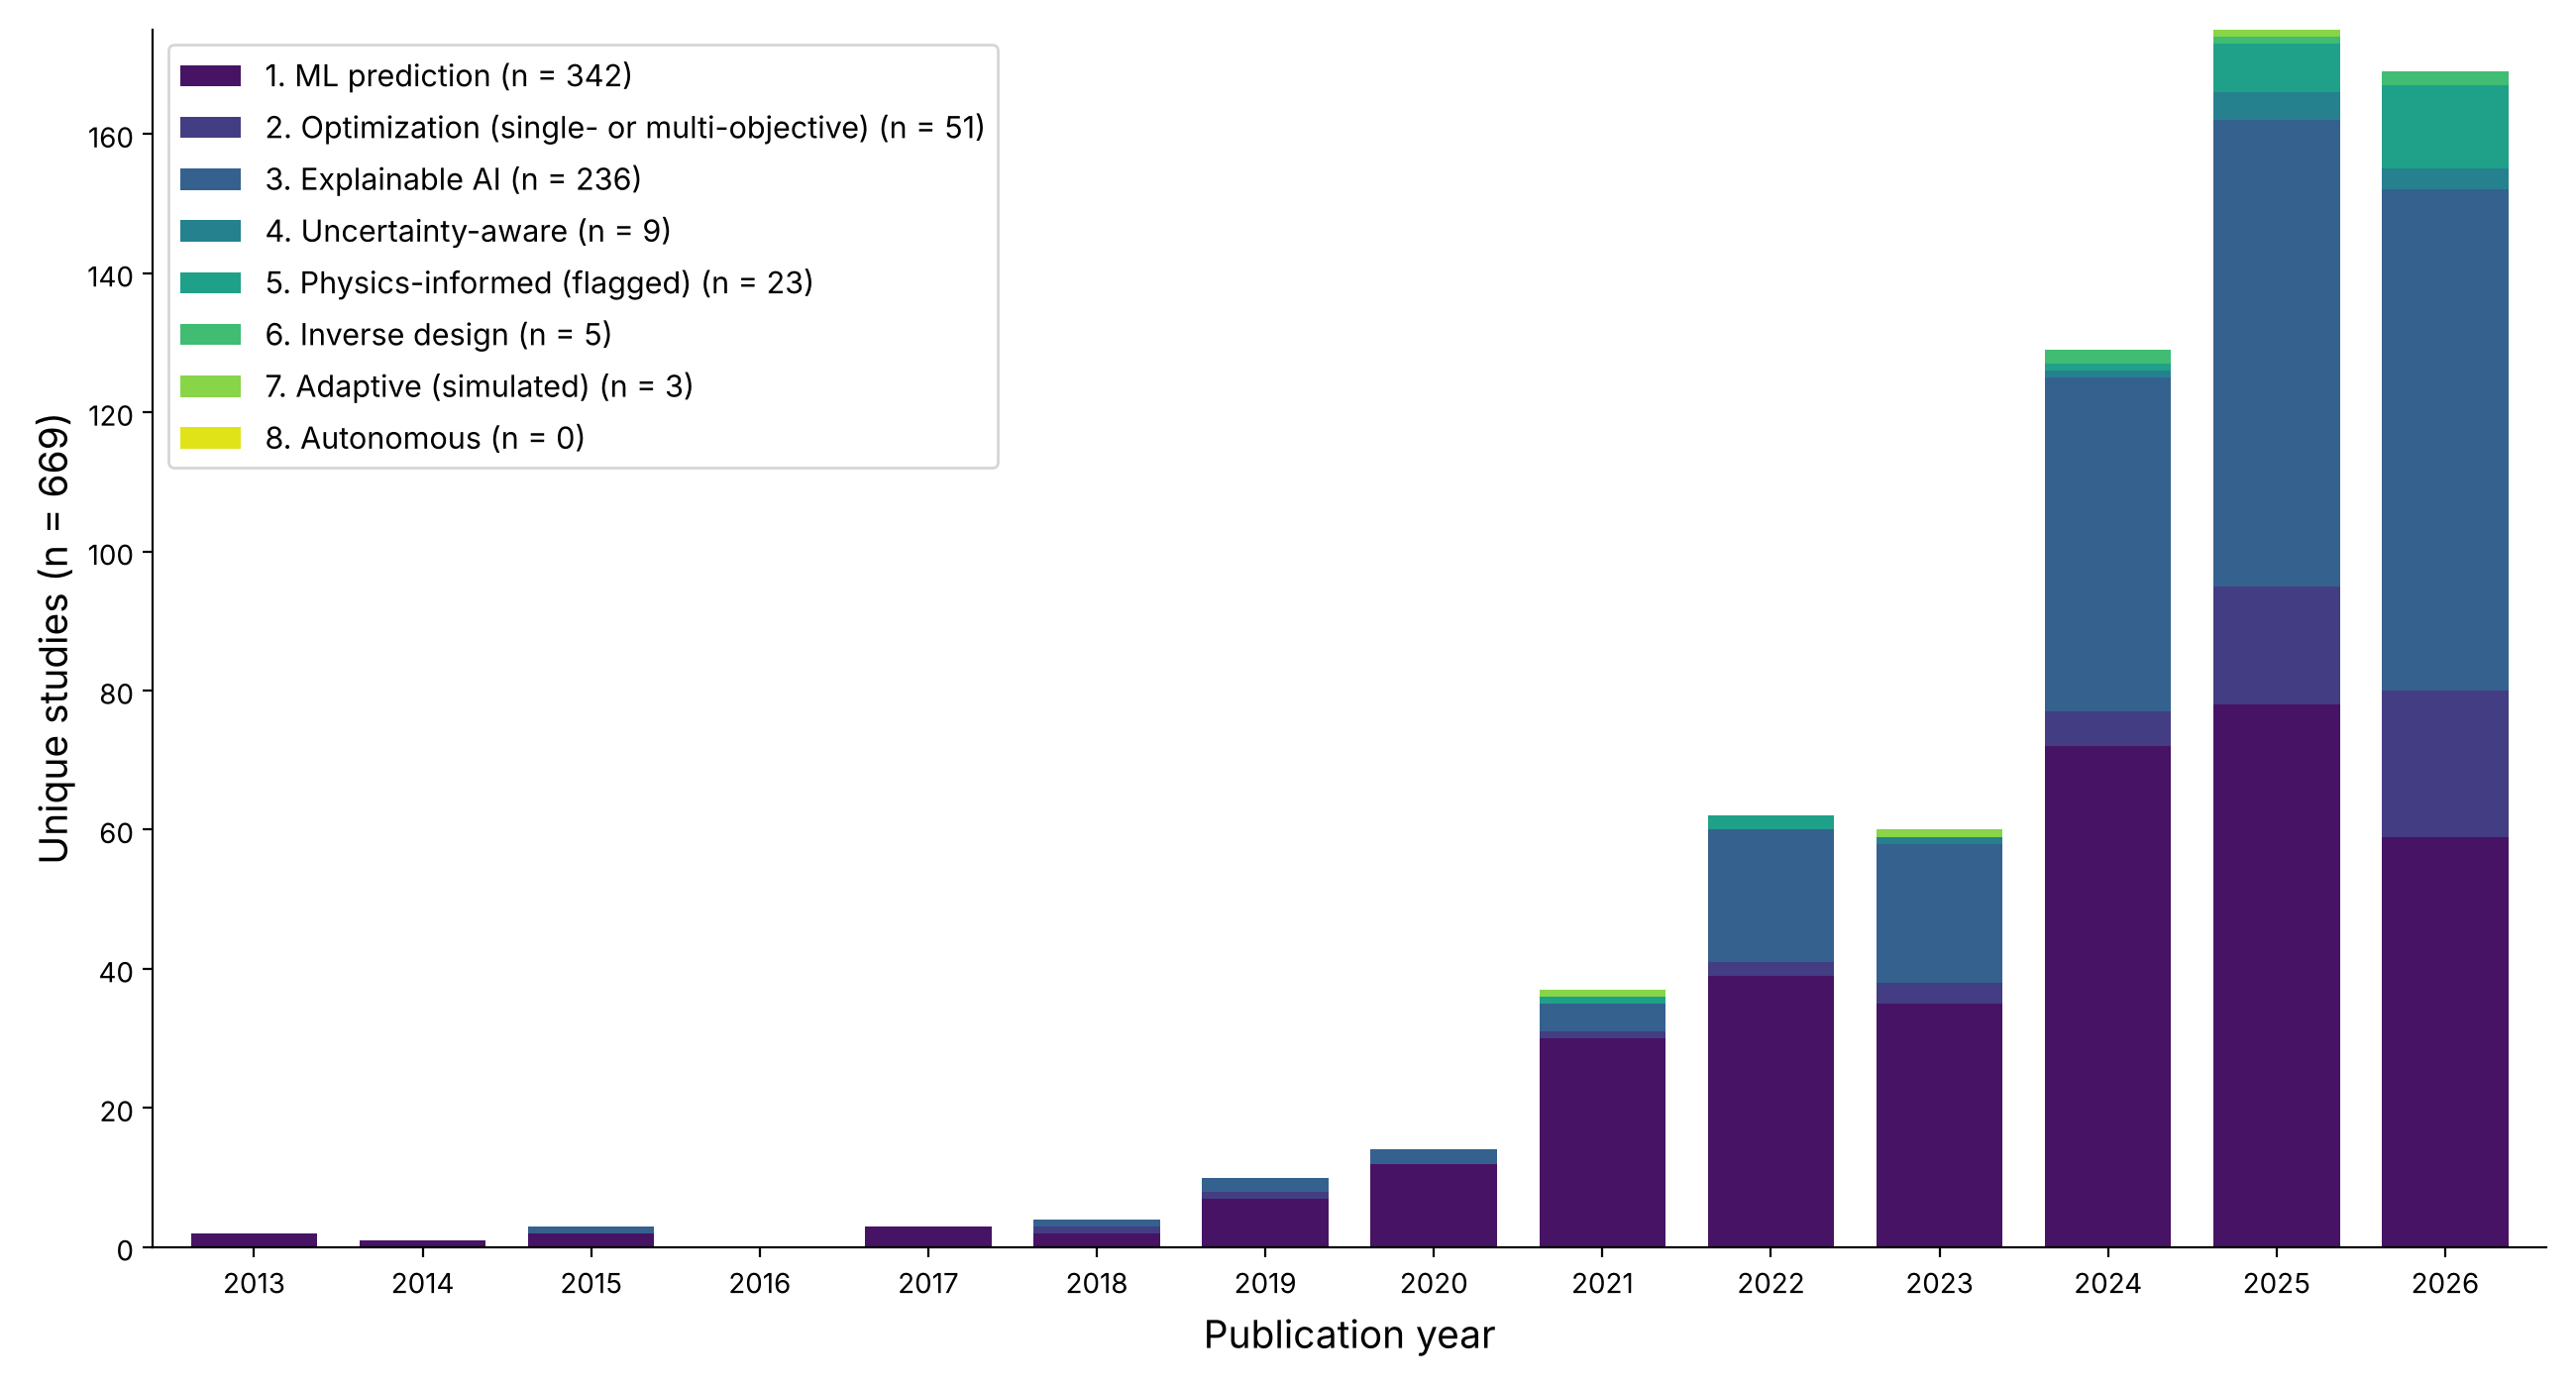
\includegraphics[width=0.95\textwidth]{Fig2.png}
\caption{Studies per year by capability stage, 2013--2026 ($n = 669$). Each study is placed at the highest stage for which its abstract carries the corresponding vocabulary (keyword classifier). ``Physics-informed'' counts flagged studies, before the audit of Section~\ref{sec:physics}. A study is counted once, at its highest stage, so stage counts differ from the single-axis totals in the text (Section~\ref{sec:framework}). The 2026 bar is incomplete (the search was run in August) and includes one article online in 2026 with a 2027 volume year}\label{fig2}
\end{figure}

\section{Findings}\label{sec:findings}

\subsection{A young, fast-growing and prediction-centred field}\label{sec:core}

The corpus contains six studies from 2013--2015, fewer than fifteen a year from 2016 to 2020 (31 in all), 37 in 2021, 62 in 2022, 60 in 2023, 129 in 2024, 175 in 2025 and 169 in the first part of 2026 (the last figure includes one article online in 2026 with a 2027 volume year). Studies published since January 2024 make up 70.7\% [95\% CI 67.1--74.0] of the total. Most appear in construction-materials journals (\emph{Construction and Building Materials} leads with 57 studies); venues from computer science are almost absent.

\emph{Materials.} Coverage follows data availability. Fly-ash/slag blends (23.8\% of studies), fly-ash systems (23.2\%) and slag systems (15.5\%) dominate, with mixed or other AAMs at 28.6\% (shares sum to more than 100\% because several labels can apply). Stabilized soils account for 6.3\%, metakaolin and calcined clays 6.1\%, biomass ashes 4.2\% and recycled-aggregate systems 3.6\%. The residues that are hardest to use and whose use would matter most are modelled least: one-part systems 2.8\%, mine tailings 1.2\% and red mud 1.2\%. The feedstocks on which models are trained are those whose supply is expected to shrink.

\emph{Inputs.} Typical model inputs are mix proportions, activator parameters, curing temperature and age, and in some studies oxide fractions. Reactive (amorphous) content, particle size and dissolution behaviour are usually missing, because compiled literature data can carry only what the source papers reported. Two studies that treat feedstock reactivity as the modelling problem show an alternative \citep{song2025,qi2022}.

\emph{Tasks.} Property prediction, and optimization built on predictive models, together account for 94.5\% [95\% CI 92.5--96.0] of the corpus. The remainder is microstructure and image analysis (3.6\%), classification (1.5\%) and experiment selection (0.4\%). Within the main family, 78.3\% of studies are prediction only and 16.1\% [13.5--19.1] use the vocabulary of mix-design optimization (10.3\%), multi-objective optimization (5.1\%) or inverse design (0.7\%). A study that tunes a predictive model with a metaheuristic, without searching a design space, is counted as prediction. The human recode gives a similar share of design work in its sample (13 of 67), although the two codings often select different studies (Section~\ref{sec:reliability}), so about 16\% is best read as an approximate figure. Supplementary Table S10 cross-tabulates material system against task.

Compressive strength, usually at 28 days, is by far the most common target. Durability targets, such as carbonation depth, chloride ingress and acid or sulfate resistance, are mentioned in 23.9\% of abstracts. Gradient-boosted trees and feed-forward neural networks are the standard models, frequently combined with metaheuristic tuning. A typical study compiles data from the literature, splits it at random, tunes by cross-validation, reports $R^2$ and error metrics and ends with a SHAP plot. This workflow has shown that composition and curing variables can predict 28-day strength well inside densely sampled ranges. It does not show how the models behave outside those ranges, which is the subject of the next sections.

\subsection{Trust: explainability is common, reliability evidence is rare}\label{sec:trust}

Table~\ref{tab:score} gives the share of studies whose abstracts carry the vocabulary of each trust practice. Explainability is signalled in 39.3\% [35.7--43.1] of studies and has risen steeply since 2022 (Fig.~\ref{fig3}); it is almost always SHAP or feature-importance analysis. The other practices are signalled far less often: external validation 4.6\% [3.3--6.5], uncertainty quantification 1.8\% [1.0--3.1], out-of-distribution or transfer evaluation 1.3\% [0.7--2.5] and calibration 0.6\% [0.2--1.5]. No abstract names a code repository. In 57.8\% [54.1--61.5] of studies no trust-practice term appears.

These figures need careful reading. They count vocabulary in abstracts. External validation and code availability in particular are often described only in the body of a paper or in a data-availability statement, so their true prevalence is higher than shown, by an amount this review did not measure. The human recode found explainability somewhat more often than the classifier did. What the data support is the contrast: explainability is now routinely advertised, and the practices that test whether a model's predictions can be relied on are not. Robustness and physical consistency cannot be assessed from keywords and are not reported.

The contrast matters because an explanation of an unvalidated model describes the model, not the material. Many of the studies read in full train on a small number of compiled literature databases (Section~\ref{sec:data}), so similar importance rankings across papers may reflect shared data more than independent confirmation.

\emph{Calibration.} Four abstracts use calibration vocabulary, and three of these studies show that the practice is inexpensive. One applies conformal prediction across thirty data splits with control of group leakage and reports empirical coverage of 89.6\% against a nominal 90\% \citep{parakhiya2026}. A companion study couples conformal intervals to gradient boosting and to an applicability-domain analysis \citep{jagad2026}. A third uses a Gaussian-process framework whose intervals track nominal coverage and which separates uncertainty due to limited data from measurement noise, attributing most of it to limited data \citep{chan2026}. These examples come from a small number of author groups.

\emph{Validation.} Where studies report external validation, the full-text examples suggest that it is often a held-out part of the same compiled database. Designs with independent data exist: one decision-support system reports a cross-validated error of 6.23 MPa and an independent-test error of 7.86 MPa \citep{natarajan2026}, and one active-learning study checks its model against newly made laboratory specimens \citep{kazemi2025}. No interlaboratory validation and no prospective validation, on mixes designed after training, were detected in the abstracts or in the studies read in full. The authors of one of the calibration studies observe that their high $R^2$ values ``mainly reflect dense interpolation'' within the experimental range \citep{jagad2026}; that caution is likely to apply widely.

\begin{table}[htbp]
\caption{Trust practices signalled in titles, abstracts and keywords (keyword classifier, $n = 669$). Values are lower bounds on true prevalence. Robustness and physical consistency cannot be assessed at this depth}\label{tab:score}
\centering
{\footnotesize
\begin{tabular}{p{0.24\textwidth}p{0.44\textwidth}rr}
\toprule
Practice & Question it answers & Studies & \% of 669 \\
\midrule
Explainability & Why did the model predict this? & 263 & 39.3 \\
External validation & Was independent data used? & 31 & 4.6 \\
Uncertainty quantification & How uncertain is the prediction? & 12 & 1.8 \\
Out-of-distribution or transfer test & Does it hold for unseen compositions? & 9 & 1.3 \\
Calibration & Are the stated ranges right as often as claimed? & 4 & 0.6 \\
Named code repository & Could another group repeat this? & 0 & 0.0 \\
None signalled & & 387 & 57.8 \\
\bottomrule
\end{tabular}}
\end{table}

\begin{figure}[htbp]
\centering
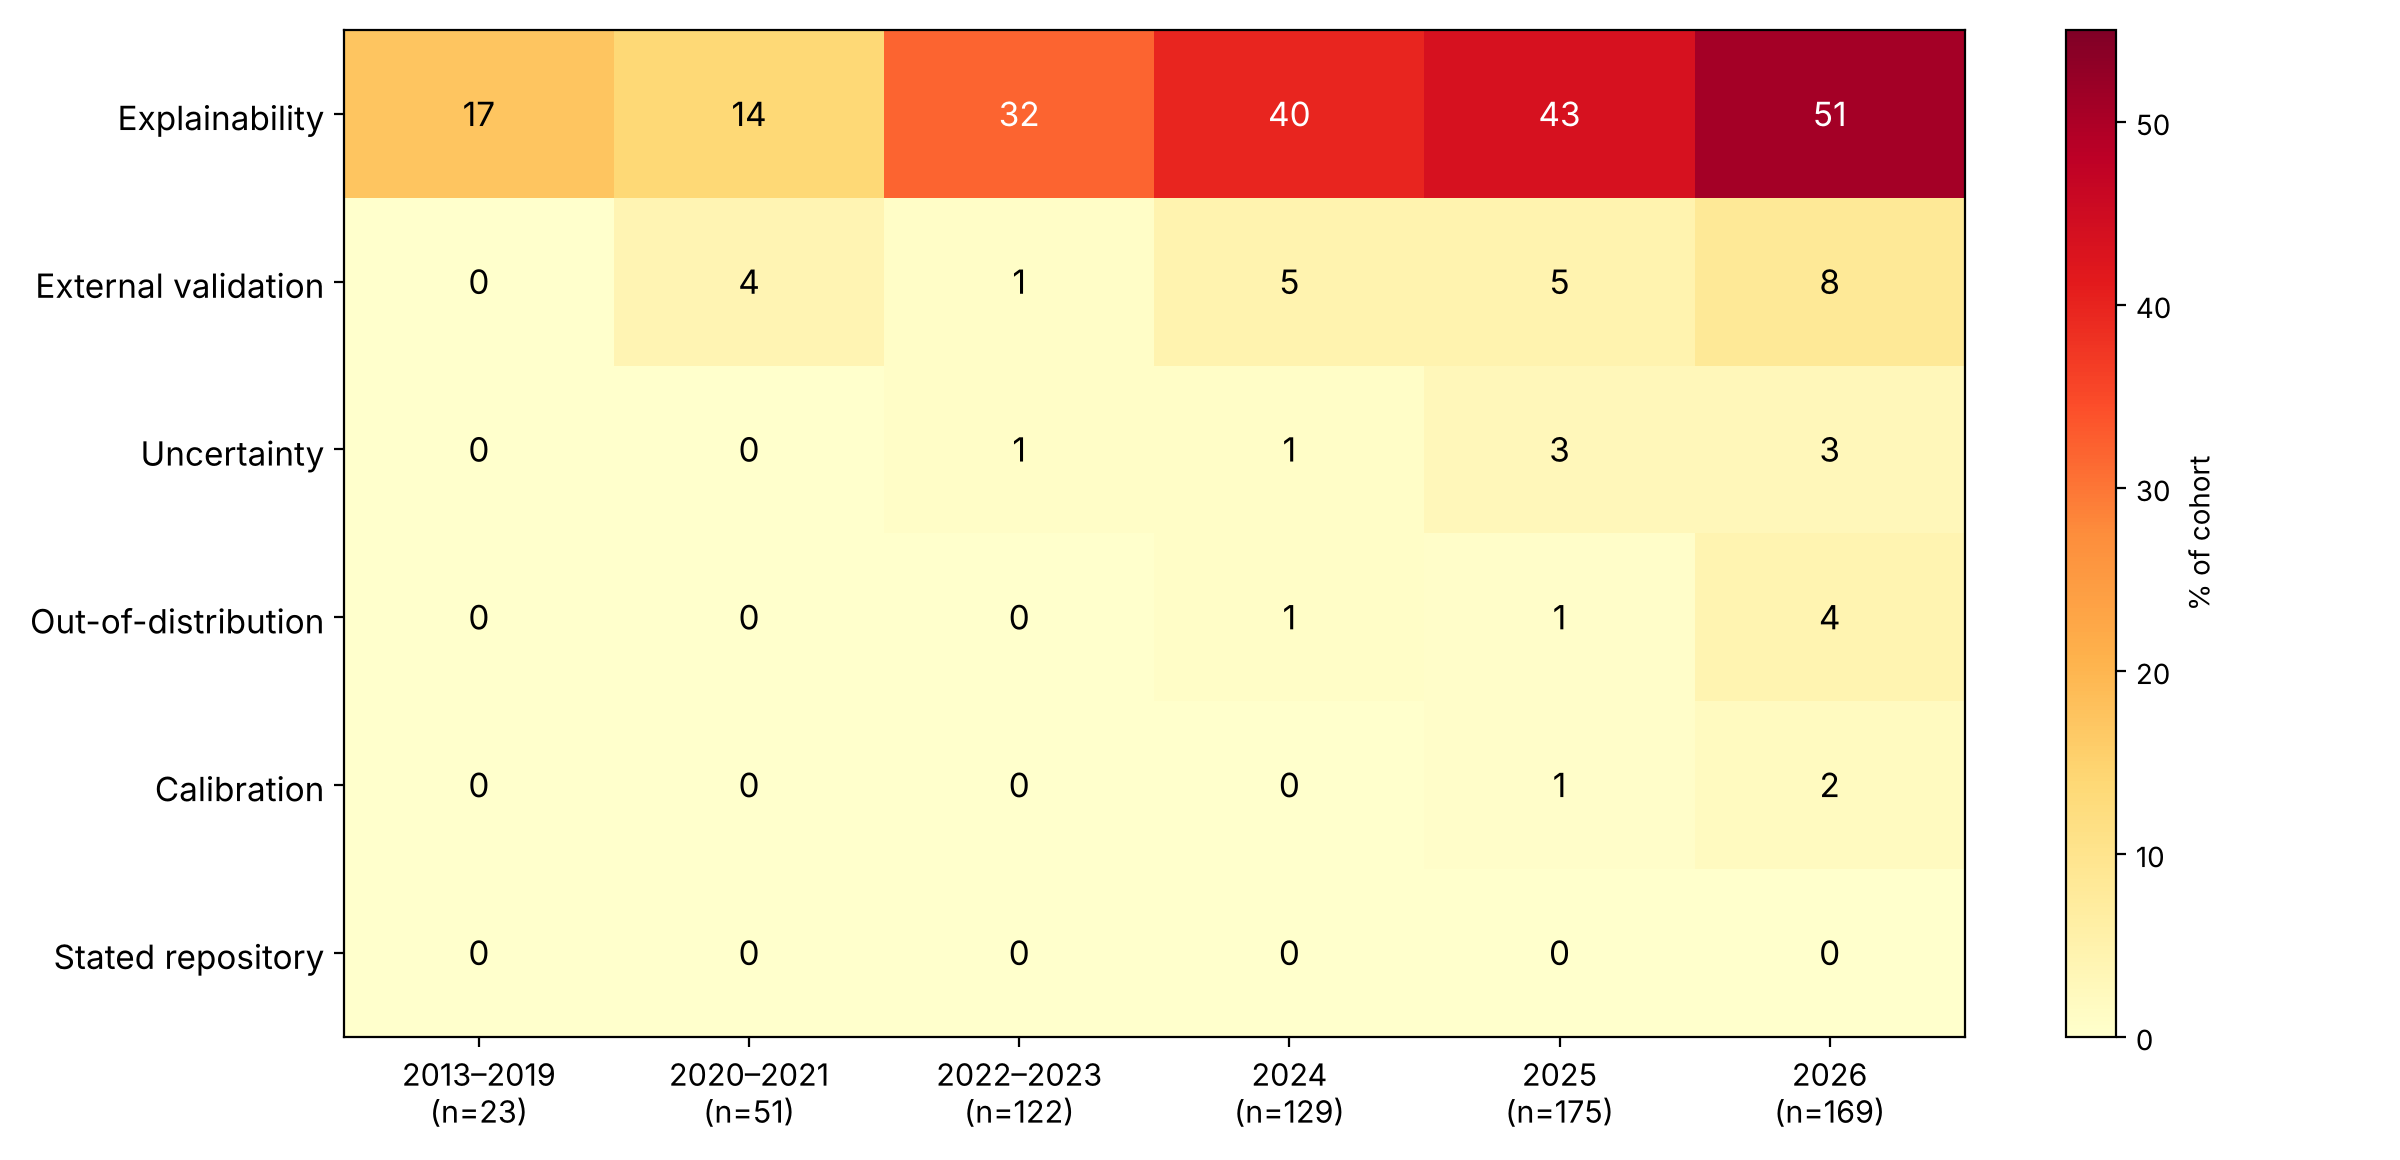
\includegraphics[width=0.9\textwidth]{Fig3.png}
\caption{Share of studies signalling each trust practice, by publication cohort (\% of cohort; keyword classifier). Cell values are rounded to whole percentages of each cohort. Early cohorts are small, so single studies move their values by several points}\label{fig3}
\end{figure}

\subsection{Physics and chemistry integration: a small verified group}\label{sec:physics}

By keyword coding, 80.3\% [77.1--83.1] of studies are Type I and 16.1\% [13.5--19.1] are Type II. The boundary between these two types is sensitive to vocabulary, but their sum, 96.4\% [94.7--97.6], is stable. The classifier flags the remaining 24 studies (3.6\%) because their abstracts use physics-informed, knowledge-guided, thermodynamic or mechanistic vocabulary.

The audit covers 32 studies: 27 assembled before the keyword coding and five added because the classifier flagged them (Section~\ref{sec:reliability}). Seventeen carry an explicit label from their authors such as knowledge-guided, chemistry-informed or physics-informed. Fifteen were included as candidates for mechanistic--ML coupling because their abstracts describe reaction mechanisms or simulation alongside ML; their authors do not necessarily describe them as physics-informed. Each of the 32 was graded against what its abstract and, where available, its methods description show (Supplementary Table S11; Supplementary Fig.~S2). Eleven were verified at Type III or above, 18 were downgraded to Types I--II and three could not be verified from the available description. Nine of the eleven model mix-level behaviour and two are machine-learned interatomic potentials working at the atomic scale. Among the 17 studies with an explicit author label, seven were verified, seven were downgraded and three could not be verified. The typical downgraded case uses oxide ratios as input features, which is sound feature engineering but is Type II. Two studies pair ML with density-functional-theory calculations that explain the result without constraining the model, and these are also downgraded. Three of the five added studies were downgraded because the word ``mechanistic'' in their abstracts refers to interpretation and not to the model, and one of them states explicitly that its model is a statistical surrogate. Two cautions apply. The grading was done by one author, mostly without the full text. And the human recode found two studies with mechanistic coupling that carry no physics vocabulary, so eleven is a minimum; those two are not among the 32.

The eleven verified studies fall into four groups, given here in the order of the type scale (Type III, Type IV, then two groups at Type V). \emph{Knowledge guidance:} knowledge graphs used to steer learning and multi-objective search for ultra-high-performance geopolymer \citep{guo2024}; a knowledge-guided ensemble for stabilized dredged sludge \citep{su2026}; and automated construction of such graphs with a large language model, applied to ultra-high-performance geopolymer design \citep{jiang2026}, the only use of a language model found in the corpus. \emph{Embedded constraints:} a carbonation-depth network with an embedded physical relation \citep{liu2025}; physics-informed neural networks that identify chloride diffusion coefficients in alkali-activated mortars \citep{wan2025}; and an equation-embedded network used as the objective in a four-objective search over strength, cost, CO$_2$ and energy \citep{guo2026}. \emph{Mechanistic hybrids:} ML combined with thermodynamic simulation to relate composition to properties \citep{ke2021}; a random-forest model constrained by network-topology and phase-assemblage information across twenty-six precursors \citep{bhat2022}; and ML combined with thermodynamic modelling for one-part AAM strength development \citep{pei2026}. \emph{Machine-learned interatomic potentials:} two studies train ML force fields on density-functional-theory data and use them inside atomistic simulation, one to characterize aluminosilicate hydrate gels \citep{li2026mlp} and one to compute dissolution activation energies for metakaolin \citep{izadifar2025}. These operate at the atomic scale and inform mechanism; they do not predict mix-level properties. No study combines two of these approaches.

Likely obstacles to wider use are the need for expertise in both chemistry and ML, the lack of any agreed vocabulary for levels of integration, and the absence of shared datasets that include reaction-relevant descriptors.

\subsection{Design and environmental assessment}\label{sec:env}

\emph{Design search.} A real body of work now asks which mix meets stated requirements, not only what strength a given mix will have. Single-objective studies usually maximize strength with a genetic or swarm algorithm over a fitted model. Multi-objective studies trade strength against cost, workability, durability or carbon. Inverse design appears as recommender systems \citep{natarajan2026}, as generative approaches \citep{gu2025} and as conformal, uncertainty-aware search restricted to the model's applicability domain \citep{jagad2026}. Three things are usually missing: uncertainty, since Pareto fronts are computed from point predictions; physical feasibility constraints beyond simple bounds; and experimental confirmation. No study reporting that an optimized mix was subsequently made, tested and fed back to the model was detected in the abstracts or in the studies read in full.

\emph{Environmental quantification.} The case for geopolymers is environmental, and most abstracts say so. By keyword coding, 40.8\% [37.1--44.6] of studies carry no term for any environmental variable (carbon, life-cycle assessment, cost, durability or waste valorization). This is a lower bound on the share that quantify none, because the classifier credits a study whenever such a term appears, whether or not a quantity is reported. The human coder, who required quantification, found no environmental variable in 69\% of the recode sample against the classifier's 52\% for the same studies. Carbon terms appear in 26.2\% of abstracts and life-cycle assessment terms in 2.7\%.

Of the 177 studies whose abstracts use carbon or life-cycle vocabulary, 77 with explicit engagement were audited individually (Fig.~\ref{fig4}; Supplementary Table S12). In 20 (26\%) the engagement is framing without numbers. In 22 (29\%) carbon is computed from per-constituent emission factors. In 20 (26\%) carbon is an optimization objective and that is the main environmental treatment. Thirteen (17\%) perform some form of LCA, and two (2.6\% of the 77; 0.3\% [0.1--1.1] of the corpus) report an assessment with explicit boundaries consistent with ISO 14040/44. In total, 25 studies place carbon inside an optimization objective, from an early general framework \citep{shobeiri2022} through studies trading strength, cost and CO$_2$ \citep{huang2023} to the four-objective study noted above \citep{guo2026}. CO$_2$ uptake by the material is almost never modelled. No author of this review is an LCA practitioner; the audit records what studies report about boundaries and data and does not judge the quality of their inventories.

The common practice multiplies mix quantities by emission factors taken from the literature and either reports or optimizes the result \citep{alfakih2024}. It has two weaknesses. Published emission factors for activators, notably sodium silicate, differ substantially with source and system boundary, and none of the audited studies propagates that variation, so an optimizer may be choosing between mixes whose carbon difference is smaller than the uncertainty of the data. For construction products these choices, including the life-cycle modules covered and the allocation of burdens to residues such as fly ash and slag, are governed by the product category rules of EN 15804 and ISO 21930 \citep{en15804,iso21930}. And when the CO$_2$ value is itself computed from the mix proportions, a model that predicts it is partly relearning that arithmetic. Optimized carbon figures from this literature should therefore be treated as screening estimates until boundaries, data sources and uncertainty are reported.

\begin{figure}[htbp]
\centering
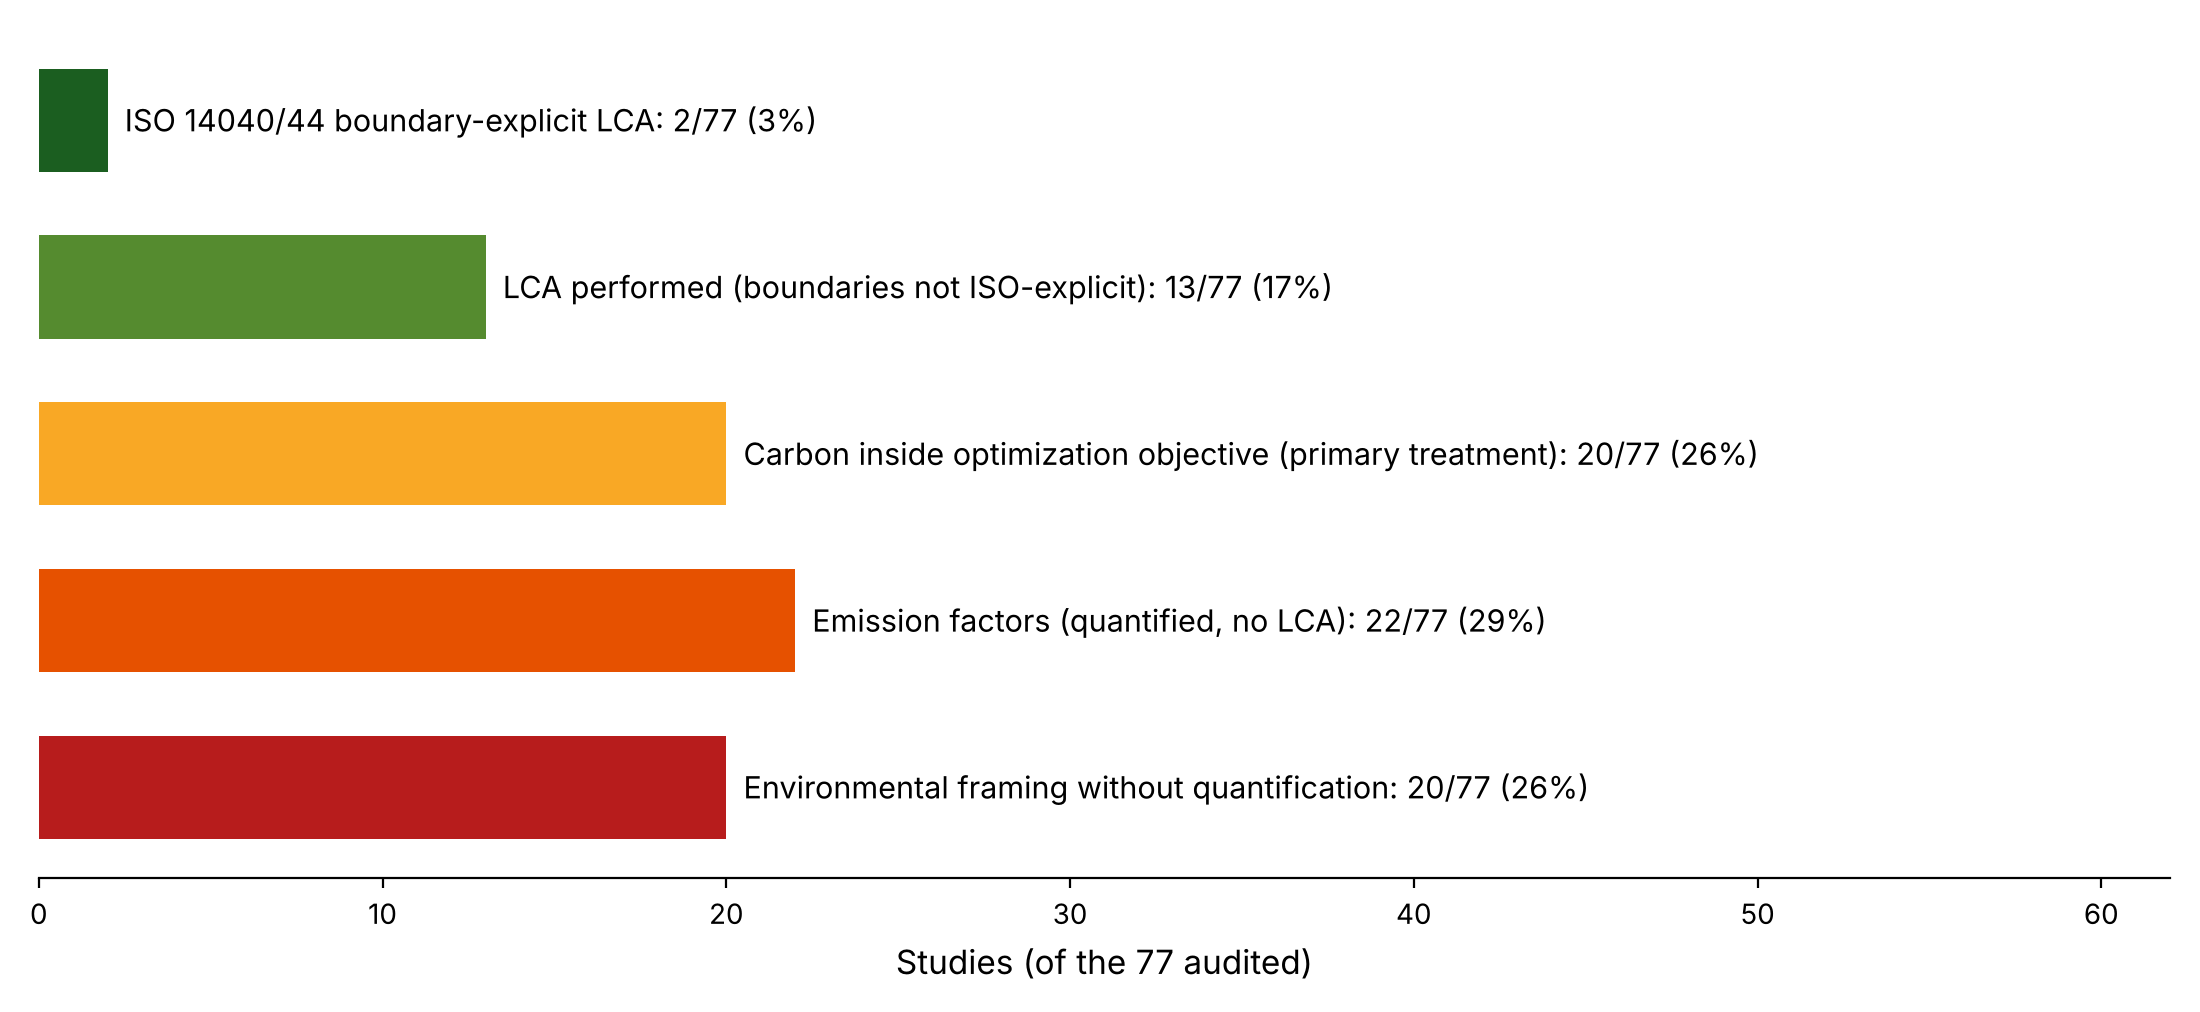
\includegraphics[width=0.9\textwidth]{Fig4.png}
\caption{Primary environmental treatment in the 77 audited studies. Categories are mutually exclusive. In total 25 of the 77 place carbon inside an optimization objective, 20 as the primary treatment shown here. Bar labels are rounded to whole percentages}\label{fig4}
\end{figure}

\subsection{Adaptive experimentation, digital twins and deployment}\label{sec:adaptive}

\emph{Adaptive experimentation.} Three studies (0.4\% [0.2--1.3]) use sequential or active learning. One benchmarks it on 131 alkali-activated binder mixtures and reports large reductions in the number of experiments needed to reach a target strength \citep{volker2021}; a second extends this to eight datasets with CO$_2$ footprint as a second objective \citep{volker2023}; a third applies active learning to alkali-activated ultra-high-performance concrete and checks its model against new laboratory tests \citep{kazemi2025}. In all three the experiments selected by the algorithm were rows of an existing dataset. The evidence that adaptive design would work for geopolymers is therefore simulated; no physical propose--make--test--update loop was detected.

\emph{Digital twins, agents and self-driving laboratories.} No digital twin of a geopolymer material, process or structure, no language-model agent that plans experiments and no self-driving laboratory was detected, either in the corpus or by the Scopus query targeting these terms. These absences hold for the English-language journal literature searched here; conference papers and preprints, where such work often appears first, were excluded. Components exist separately: acoustic-emission monitoring of early-age reaction \citep{jin2024}, physics-informed transport models \citep{wan2025}, and a model that updates later-age strength predictions from early-age measurements \citep{chan2026}. Two 2026 studies bring foundation models into the field, a tabular foundation model evaluated on out-of-range data \citep{zhang2026} and the language-model knowledge-graph work \citep{jiang2026}; both are tools operated by people. Self-driving laboratories are established in other areas of chemistry and materials science \citep{tom2024}. Plausible reasons they have not reached AAMs are the 28-day verification time, batch-to-batch feedstock variation, the handling of viscous activator solutions and the lack of calibrated models to steer a loop. One-part dry-mix formulations and early-age updating models address two of these.

\emph{Deployment.} On the deployment axis most studies end at laboratory prediction, a minority reach formulation recommendation, and a few offer decision-support tools \citep{natarajan2026,kazemi2025}. No process-control implementation, pilot project using model-guided mixes, or engagement with certification or standards bodies was detected. Construction codes are largely prescriptive and written for Portland cement. Performance-based acceptance, which some jurisdictions allow in limited form, is the route by which a model output could enter practice (existing examples are the performance specification for hydraulic cement, ASTM C1157, and the British specification for alkali-activated cementitious material and concrete, PAS 8820; \citealp{astmc1157,pas8820}): a prediction with a verified uncertainty range could reduce, though not replace, physical testing. An uncalibrated model cannot play that role, which is why the trust findings of Section~\ref{sec:trust} bear directly on deployment.

\subsection{Data, validation and reproducibility}\label{sec:data}

\emph{Data.} Among the studies read in full, the usual data source is a compilation of mixes from earlier papers, of roughly one hundred to nine hundred records, and the same compilations recur under different models. How widespread this reuse is across the whole corpus was not measured, because data provenance is rarely stated in abstracts. Reuse has consequences: many models trained on one dataset are not independent evidence, and errors in a dataset propagate. One study removed 37 duplicate records from a 594-record compilation before modelling \citep{parakhiya2026}. Larger curated compilations exist, notably an open dataset of more than a thousand alkali-activated concrete formulations and their properties \citep{morenotorres2023} that accompanies one of the adaptive-design studies \citep{volker2023}, but no shared benchmark with fixed, leakage-safe splits exists. This review met the same problem in its own corpus (Section~\ref{sec:dup}).

\emph{Validation and leakage.} Random splitting of compiled data is the norm in the studies read in full. It allows near-identical mixes from one laboratory series to fall in both training and test sets. One study guards against this by keeping identical feature vectors together \citep{parakhiya2026}. Group-aware splitting and declaration of an applicability domain are routine in cheminformatics and could be adopted directly. A further low-cost test is available: train on studies published before 2024 and test on those published since.

\emph{Reproducibility.} No abstract names a code repository, and none of the 16 studies read in full gave a resolvable one. Because repositories are usually cited in the body of a paper, the true rate is uncertain; the available evidence suggests it is low. During screening, one retraction notice was found among the records. Nothing currently removes retracted results from compiled datasets.

\emph{Unresolved disagreements.} Four tensions in the literature mark where evidence is thin (Supplementary Table S13). Generative data augmentation is reported to help in one study \citep{gu2025} and to reduce accuracy in another \citep{liu2025}, and most augmentation studies do not test on real data only. Feature-importance rankings agree across many studies, but possibly because data are shared. Claims that a particular algorithm is best rest on comparisons across different datasets. And 25 studies optimize carbon while two assess it with explicit boundaries.

\section{Research gaps and roadmap}\label{sec:gaps}

The findings are summarized as nine gaps, each with the evidence for it and a test that would show it closed (Table~\ref{tab:gaps}). The gaps depend on one another. Shared, well-documented data (G6) is needed before reliability can be established (G1, G2, G7); reliability is needed before deployment (G8); physics integration (G3) and environmental quantification (G4) make reliable models useful for clean technology; and automation (G5) would amplify whatever weaknesses remain in the models that steer it. The disagreement over data augmentation (G9) can be settled only on shared data with real-only test sets (G6, G7). Supplementary Fig.~S3 shows these dependencies. The roadmap follows this order (Table~\ref{tab:roadmap}; Fig.~\ref{fig5}). Its horizons are our judgment and are indicative.

\begin{table}[htbp]
\caption{Nine research gaps, the evidence for each and the test that would show it closed. Percentages are keyword-classifier shares of 669 studies}\label{tab:gaps}
\centering
{\footnotesize
\begin{tabular}{p{0.19\textwidth}p{0.37\textwidth}p{0.33\textwidth}}
\toprule
Gap & Evidence in this review & Closed when \\
\midrule
G1 Calibration & Uncertainty signalled in 1.8\%, calibration in 0.6\%, from few groups & Coverage verified on newly made mixes \\
G2 Interpolation & Random splits of compiled data; applicability domain rarely declared & Leave-one-source-out results and a blind interlaboratory test \\
G3 Physics integration & 32 studies audited, 11 verified, 18 downgraded, 3 not verifiable & Constraint-violation checks and ablations showing the physics contribution \\
G4 Environmental quantification & At least 41\% mention no environmental variable; 2 boundary-explicit LCAs; factor uncertainty not propagated & ``Low-carbon'' designs carry a boundary-explicit assessment and one physical verification \\
G5 Closed loops & 3 adaptive studies, all simulated; no twin, agent or physical loop detected & Two consecutive physical propose--make--test--update cycles \\
G6 Data infrastructure & Reused compilations; duplicates documented; no shared benchmark & Three independent groups report on identical splits \\
G7 External validation & Signalled in 4.6\%; no interlaboratory or prospective test detected & Error reported from cross-validation through to prospective test \\
G8 Deployment & No pilot, certification or standards engagement detected & One AI-designed mix accepted through a performance-based process \\
G9 Augmentation & Contradictory results; few real-only test sets & Benefit shown on real-only test data \\
\bottomrule
\end{tabular}}
\end{table}

\textbf{Immediate (0--2 years): make existing models honest.} None of these needs new laboratory work. (I1) A community benchmark with documented provenance, duplicate checks and fixed, leakage-safe splits, including oxide composition and environmental inventory fields; the corpus released here can serve as a starting list of sources and existing open compilations \citep{morenotorres2023} as a starting dataset. (I2) Calibration by default: conformal intervals and coverage reported beside $R^2$. (I3) Applicability-domain reporting with group-aware splits. (I4) Shared terminology: the Type I--V scale and the simulated-versus-physical label for adaptive studies. (I5) A time-split test, training on pre-2024 studies and testing on later ones.

\textbf{Emerging (2--5 years): couple models to chemistry and carbon.} (E1) Physics-constrained models used inside design search, with ablations. (E2) ML combined with LCA, using regional inventories for the main precursors and activators and carrying emission-factor uncertainty into the Pareto front. (E3) An interlaboratory round-robin on one blind set of mixes. (E4) Early-age updating models to shorten the verification cycle. (E5) A controlled test of data augmentation on the shared benchmark.

\textbf{Frontier (5--10 years): close the loop.} (F1) A first geopolymer self-driving laboratory, most feasibly on one-part dry mixes. (F2) A digital twin of curing or durability for one instrumented pilot element. (F3) Language-model tools for tasks whose output can be checked, such as extracting inventory data from papers. (F4) Models pre-trained across precursor chemistries and adapted to local residues, with stated out-of-range performance.

\textbf{In parallel: deployment and governance.} (D1) Performance-based acceptance protocols that accept a predicted property with a verified uncertainty range and a conformity-testing plan. (D2) Digital material passports recording feedstock provenance, composition, life-cycle inventory and the model's validity range. (D3) A sequence of demonstrations, from precast elements to structural pilots, each publishing predicted against measured performance.

\begin{table}[htbp]
\caption{Staged roadmap: priorities, the gaps they address and their acceptance tests}\label{tab:roadmap}
\centering
{\footnotesize
\begin{tabular}{llp{0.33\textwidth}lp{0.28\textwidth}}
\toprule
ID & Horizon & Priority & Gap & Acceptance test \\
\midrule
I1 & 0--2 y & Shared benchmark with provenance & G6 & three groups on identical splits \\
I2 & 0--2 y & Calibration by default & G1 & coverage reported beside $R^2$ \\
I3 & 0--2 y & Applicability-domain reporting & G2, G7 & validity range declared \\
I4 & 0--2 y & Shared terminology & G3, G5 & labels used in reporting \\
I5 & 0--2 y & Time-split validation & G7 & forward error published \\
E1 & 2--5 y & Physics-constrained design search & G3 & violation check and ablation \\
E2 & 2--5 y & ML--LCA with factor uncertainty & G4 & explicit boundaries on claims \\
E3 & 2--5 y & Interlaboratory round-robin & G2, G7 & public blind-set results \\
E4 & 2--5 y & Early-age updating & G5, G1 & shorter verified qualification \\
E5 & 2--5 y & Augmentation test & G9, G6 & benefit on real-only test data \\
F1 & 5--10 y & First self-driving laboratory & G5 & two physical closed cycles \\
F2 & 5--10 y & Digital-twin pilot & G5, G3 & predicted versus measured on a pilot element \\
F3 & 5--10 y & Language-model support tools & G4, G6 & audited extracted inventories \\
F4 & 5--10 y & Transferable models & G2, G6 & stated out-of-range bounds \\
D1 & parallel & Performance-based acceptance & G8, G1 & one AI-designed mix approved at pilot scale \\
D2 & parallel & Digital material passports & G8, G4, G6 & schema used in a procurement pilot \\
D3 & parallel & Demonstration sequence & G8, G7 & published predicted-versus-measured record \\
\bottomrule
\end{tabular}}
\end{table}

\begin{figure}[htbp]
\centering
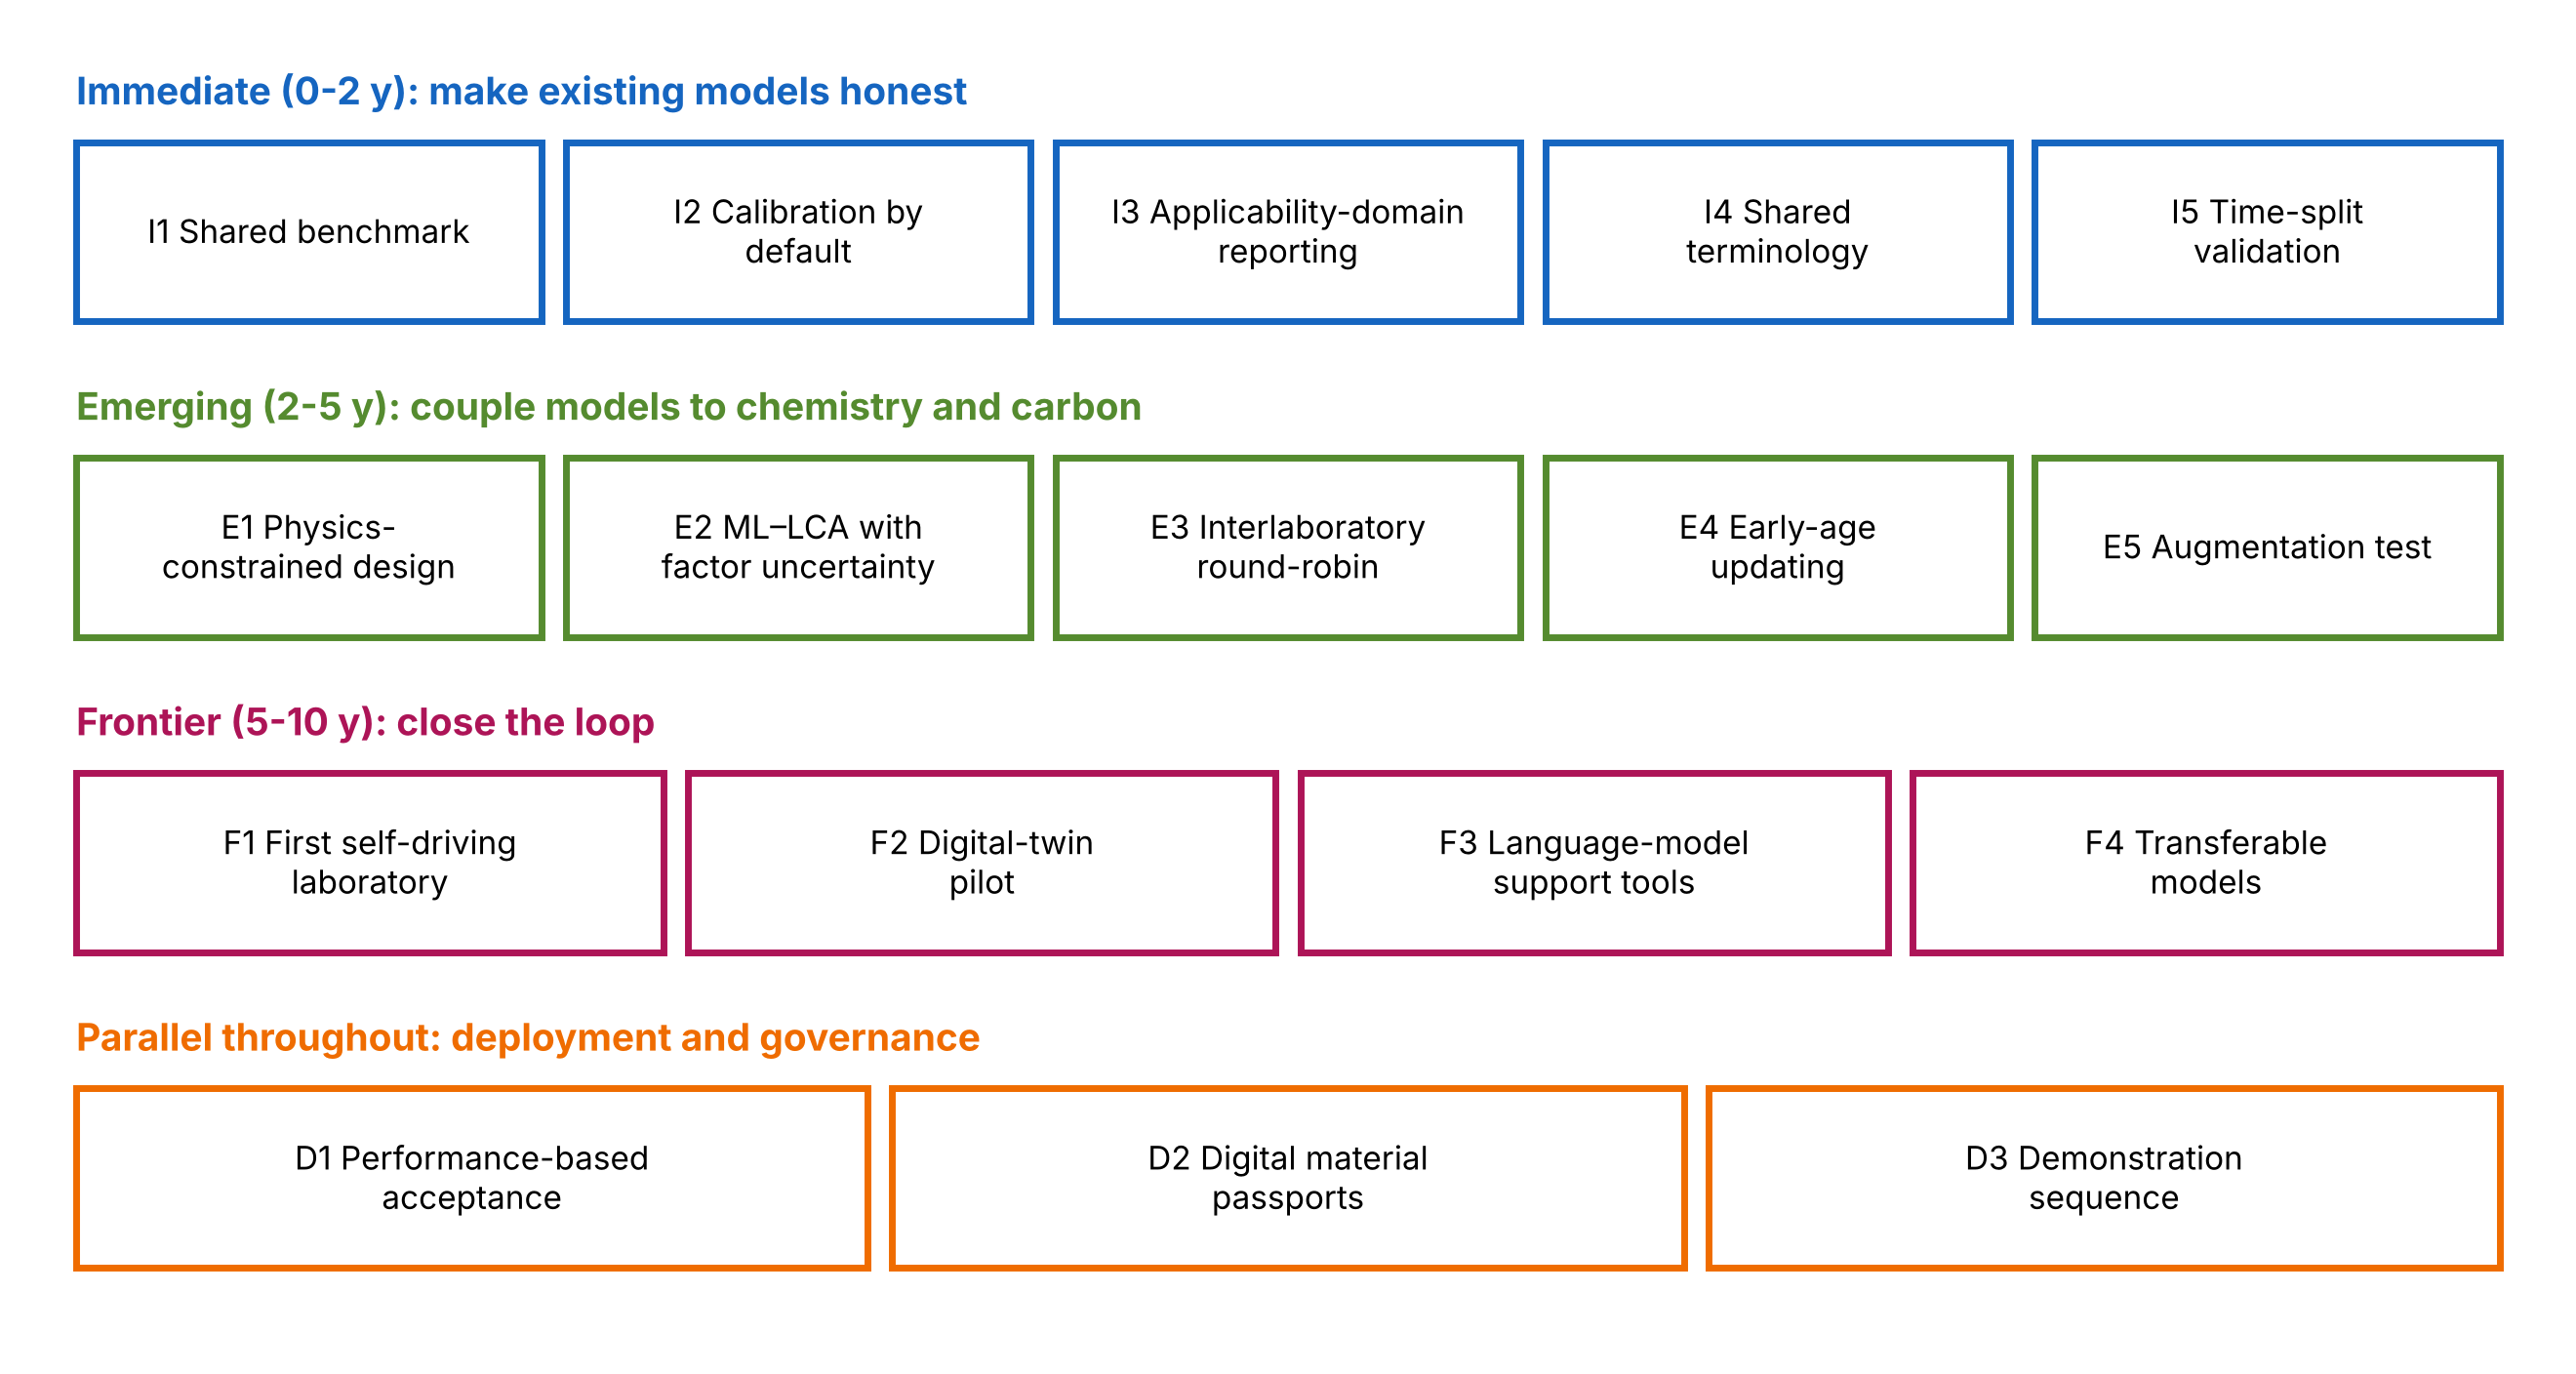
\includegraphics[width=0.95\textwidth]{Fig5.png}
\caption{The roadmap: three staged tiers and a parallel deployment and governance track. Horizons are indicative}\label{fig5}
\end{figure}

\section{Implications for policy and practice}\label{sec:policy}

The findings point to actions by three groups, none of which depends on new science.

\emph{Journals and reviewers} can act now. A short reporting checklist for AI studies of construction materials would cover data provenance and availability, how data were split and how leakage was controlled, the model's validity range, calibration results beside accuracy, the basis of any environmental figure and code release. Such a checklist can build on existing guidance for ML in concrete science and for ML-based science \citep{li2022,kapoor2024}. A disclosure rule for environmental claims would ask any manuscript describing its result as low-carbon or sustainable to state whether the claim rests on no quantification, on emission factors with sources, or on an LCA with boundaries.

\emph{Funders and the research community} can support the shared benchmark, including its maintenance: versioning, duplicate checks, credit for contributors and removal of retracted data. An interlaboratory round-robin is a modest investment that would give the field its first measured real-world error.

\emph{Standards bodies and regulators}, including RILEM, ASTM and CEN committees, can consider what evidential status a model prediction with a verified uncertainty range should have within performance-based acceptance, and under what declared validity range. Digital material passports for AAM products fit current developments in construction-products regulation, and the environmental data in them would need to follow the product category rules for environmental product declarations \citep{en15804,iso21930}. For policy makers considering AAMs in procurement or carbon accounting, the practical message is that carbon figures produced by AI-based mix optimization in the current literature are mostly screening estimates and should not be used as declared values without a boundary-explicit assessment.

\section{Limitations}\label{sec:limits}

\emph{Coding depth.} The corpus-wide statistics come from titles, abstracts and keywords. Practices reported only in full text are missed, most of all external validation and code availability, so trust-practice shares are lower bounds. The size of this under-detection was not measured; coding a random sample of full texts is the most useful next step and would allow the shares to be corrected. Statements that something was not detected rest on abstracts for the whole corpus, on the 16 studies read in full and, for digital twins and autonomy, on a dedicated query; they are not proof of absence.

\emph{Keyword coding.} The corpus-wide codes come from a keyword-heuristic classifier and not from human reading. It is deterministic and fully reproducible, but it is sensitive to vocabulary and cannot judge whether a term reflects a demonstrated practice. Against a blind human recode of 67 studies it reproduced the fine-grained labels only moderately ($\kappa = 0.25$--0.70; Section~\ref{sec:reliability}), it is more lenient than a human reader on the environmental axis, and for 12 studies the abstract came from an open index or the publisher page and lacks the index keywords that the Scopus records carry. The deployment axis, robustness and physical consistency could not be coded at all. Conclusions are therefore restricted to aggregate patterns that the human recode reproduces. The confidence intervals do not include classification uncertainty, and the recode sample is small for rare categories.

\emph{Audits.} The physics and environmental audits were reviewed by one author, largely from abstracts and methods descriptions, and were not independently repeated. Five of the 32 physics studies were added after the keyword coding and graded from their abstracts alone. Three physics-integration cases could not be verified. The two mechanistic studies found by the human recode were not added to the physics audit. Fifteen of the 32 audited studies were flagged by us, not labelled by their authors, so the share downgraded should not be read as a rate of overstatement by authors. The 77 environmentally engaged studies were selected by the first author's judgment of the abstracts, and four rows of the audit tables were corrected after a check against the abstracts. No author is an LCA practitioner.

\emph{Coverage.} Scopus was the only primary index and Web of Science was not searched. The SpringerLink harvest was truncated, although a sample check found no new eligible studies. Only English-language journal articles were included, which excludes conference papers, preprints and literature in other languages; this is most likely to affect the findings on adaptive and autonomous methods. The method terms of the core query are general, so studies that name only a specific algorithm may have been missed, and the Crossref harvest was truncated without a sample check. Citation searching and an updated search have not been done. The search ended in August 2026, so 2026 is incomplete.

\emph{Screening.} The primary screen was performed by the first author (Section~\ref{sec:reliability}); every screening decision was independently verified by a co-author. Agreement was imperfect ($\kappa = 0.83$ and 0.69), and the recode sample suggests that roughly 4--9\% of included records may be ineligible. One record was confirmed as a review, and removed, only when its abstract was retrieved; others like it may remain. Six flagged records are retained, and removing them does not change the headline figures materially. Fifty-nine duplicate reports were found only after the corpus was frozen, seven of them in a second check.

\emph{Examples and judgment.} The studies named as good practice were chosen by the authors and come from a small number of groups. The framework, the scorecard and the roadmap horizons are constructed instruments, and other reasonable constructions exist. Two authors of this review co-authored one study in the corpus (see Competing interests).

\emph{Currency.} In a field where most studies are less than three years old, the shares reported here will date quickly. The released corpus allows them to be recomputed.

\section{Conclusions}\label{sec:concl}

Across 669 journal studies, AI research on geopolymers is overwhelmingly concerned with predicting properties and optimizing over those predictions. A design-search literature has emerged, about 16\% of studies, and it increasingly includes carbon among its objectives. The evidence that would let these models support engineering or policy decisions is much thinner. In abstracts, explainability is common while calibration, external validation and code release are rarely signalled; only eleven studies were verified as building physics or chemistry into the model, nine of them at mix level; at least 41\% of studies mention no environmental variable and two report a boundary-explicit LCA; and no physical closed loop, digital twin or certification pathway was detected. These figures come from keyword coding of abstracts and several are lower bounds, but the overall pattern does not depend on any single one of them.

Each weakness is matched by at least one study in the corpus that shows how to address it, through conformal calibration, applicability-domain declaration, thermodynamic or constraint-embedded models, boundary-explicit LCA or early-age updating. The task is therefore one of adoption. The order proposed is shared data and reliability reporting first, coupling to chemistry and carbon next, closed experimental loops after that, with acceptance frameworks developed in parallel. Until models are validated beyond their training data and their carbon figures are assessed, the contribution of AI to low-carbon construction through geopolymers is a prospect that the current literature has not yet demonstrated.

\backmatter

\bmhead{Supplementary information}
Supplementary Materials accompany this article: Table S1 (PRISMA reconciliation), Note S7 (SpringerLink sample screen), Table S8 (confidence intervals), Table S9 (coding reliability against the human recode), Table S10 (material system by task), Table S11 (physics-integration audit), Table S12 (carbon and LCA audit), Table S13 (tensions in the literature), Table S14 (classifier sensitivity and specificity against the human recode) and Figures S1--S3 (framework diagram, physics-audit outcome, gap dependencies). Items S2 (query strings), S4 (taxonomy candidates and coding rules) and S6 (full gap chains) are files in the research artifact; the numbers S3 and S5 are not used.

\bmhead{Acknowledgments}
The authors thank the maintainers of the open databases and open-access publications on which this synthesis depends.

\section*{Declarations}

\bmhead{Funding}
The authors declare that no funds, grants, or other support were received during the preparation of this manuscript.

\bmhead{Competing interests}
Two authors of this review (V.N. and S.S.A.) are authors of one primary study in the corpus: Nageshwaran V, Amritphale SS, Ezekiel S (2026) Interpretable machine learning for one-part fly-ash/slag geopolymer strength prediction: Toward multifunctional binder design, Materials 19:3347, \url{https://doi.org/10.3390/ma19153347}. It entered the corpus under the same criteria as all other studies, and both its primary screener and its assigned verifier were among its authors. A co-author who is not an author of that study (P.K.C.) has independently confirmed its eligibility. The study is not part of the physics audit, the carbon audit or the 16 studies read in full. Its eligibility can be checked from its published metadata; it is not cited as an example in this review. The authors have no other relevant financial or non-financial interests to disclose.

\bmhead{Data availability}
The research artifact (screening ledger with per-record decision codes, coded corpus of 728 records and 669 unique studies with duplicates flagged, duplicate-audit evidence, audit tables, recode worksheets, extraction files, the keyword classifier with its lexicon and output, and scripts) is archived at Zenodo (\url{https://doi.org/10.5281/zenodo.22325910}) and maintained at \url{https://github.com/vnageshwaran-de/ai-geopolymer-prisma-corpus}.

\bmhead{Author contributions}
VN: conceptualization, methodology, software, formal analysis, investigation, data curation, writing --- original draft, visualization. PKC: validation (independent screening; blind coding-reliability recode; environmental-claims review), investigation, writing --- review and editing. SSA: validation (independent screening; geopolymer-science review), resources, writing --- review and editing, supervision. MD: supervision, writing --- review and editing. All authors read and approved the final manuscript.

\bmhead{Ethics approval}
Not applicable; this study involved no human participants or animals.

\bibliography{sn-bibliography}

\end{document}
